\documentclass[11pt,a4paper]{article}

% ---------------- Matematica (Palatino, stile manuale scientifico) ----------------
\usepackage{amsmath,amssymb,mathtools}
\usepackage[sc]{mathpazo}
\usepackage{bm}
\linespread{1.06}

% ---------------- Font del testo ----------------
\usepackage[no-math]{fontspec}
\setmainfont{TeX Gyre Pagella}
\setsansfont{Fira Sans}[BoldFont={Fira Sans SemiBold},ItalicFont={Fira Sans Italic},BoldItalicFont={Fira Sans SemiBold Italic}]
\newfontfamily\headfont{Fira Sans}[BoldFont={Fira Sans SemiBold},ItalicFont={Fira Sans Italic}]
\newfontfamily\headlight{Fira Sans Light}
\newfontfamily\headblack{Fira Sans ExtraBold}

\usepackage{babel}
\babelprovide[import,main]{italian}

% ---------------- Pagina ----------------
\usepackage[a4paper,top=2.5cm,bottom=2.4cm,left=2.3cm,right=2.3cm,headheight=15pt,headsep=0.9cm]{geometry}
\usepackage[table]{xcolor}
\usepackage{graphicx,tikz,booktabs,array,tabularx,enumitem,ragged2e,pifont,microtype}
\usetikzlibrary{calc,positioning,shapes.geometric,arrows.meta,shadows}
\usepackage[most]{tcolorbox}
\usepackage{titlesec,fancyhdr,tocloft}
\usepackage[hidelinks]{hyperref}

\setlength{\parindent}{0pt}
\setlength{\parskip}{5pt plus 1pt}
\raggedright
\setlength{\RaggedRightParindent}{0pt}
\emergencystretch=2em

% ---------------- Palette ----------------
\definecolor{navy}{HTML}{1F3A5F}
\definecolor{teal}{HTML}{1B8A8A}
\definecolor{blu}{HTML}{2A6FDB}
\definecolor{rosso}{HTML}{E0533D}
\definecolor{ambra}{HTML}{D9940F}
\definecolor{viola}{HTML}{6B4FBB}
\definecolor{verde}{HTML}{2E9E5B}
\definecolor{grigio}{HTML}{5A6170}
\definecolor{chiaro}{HTML}{EEF2F7}
\definecolor{testo}{HTML}{22262D}
\color{testo}

% vettori in grassetto
\newcommand{\x}{\mathbf{x}}
\newcommand{\vv}{\mathbf{v}}
\newcommand{\mmu}{\bm{\mu}}
\newcommand{\SSigma}{\bm{\Sigma}}
\newcommand{\argmax}{\operatorname*{arg\,max}}
\newcommand{\T}{^{\mathsf{t}}}
\newcommand{\hl}[1]{{\color{navy}\bfseries #1}}
\newcommand{\key}[1]{\textcolor{teal}{\textbf{#1}}}
\newcommand{\slide}[1]{{\headfont\footnotesize\color{grigio}\,[slide #1]}}

% ---------------- Liste ----------------
\setlist{itemsep=2pt,topsep=3pt,parsep=0pt}
\setlist[itemize,1]{label={\color{teal}\small$\blacktriangleright$},leftmargin=1.3em}
\setlist[itemize,2]{label={\color{ambra}\footnotesize$\bullet$},leftmargin=1.2em}
\setlist[enumerate,1]{label={\headfont\bfseries\color{navy}\arabic*.},leftmargin=1.6em}

% ---------------- Icone (tikz) ----------------
\newcommand{\iconbulb}{\tikz[baseline=-0.6ex,scale=.85]{\fill[white](0,.06)circle(.13);\fill[white](-.07,-.15)rectangle(.07,-.06);\draw[white,line width=.4pt](-.06,-.19)--(.06,-.19);}}
\newcommand{\iconwarn}{\tikz[baseline=-0.6ex]{\node[regular polygon,regular polygon sides=3,fill=white,inner sep=1.1pt,minimum size=11pt]{}; \node[font=\headblack\tiny,text=rosso] at (0,-.02){!};}}
\newcommand{\iconml}{\tikz[baseline=-0.6ex,scale=.8]{\foreach \y in {-.16,.16}{\fill[white](-.2,\y)circle(.05);} \foreach \y in {-.2,0,.2}{\fill[white](.2,\y)circle(.05);\draw[white,line width=.35pt](-.2,.16)--(.2,\y);\draw[white,line width=.35pt](-.2,-.16)--(.2,\y);}}}

% ---------------- Box ----------------
\tcbset{every box/.style={halign=flush left}}
\tcbset{
  base/.style={enhanced,breakable,arc=3pt,boxrule=0pt,left=11pt,right=11pt,top=9pt,bottom=8pt,
    before skip=12pt,after skip=12pt,fonttitle=\headfont\bfseries\small,
    attach boxed title to top left={xshift=10pt,yshift=-9pt},
    boxed title style={arc=2.5pt,boxrule=0pt,left=6pt,right=6pt,top=2pt,bottom=2pt},
    overlay unbroken and first={}},
}
\newtcolorbox{intuizione}[1][Intuizione]{base,colback=teal!6,colbacktitle=teal,coltitle=white,
  borderline west={3pt}{0pt}{teal},title={\iconbulb\ \ #1},top=13pt}
\newtcolorbox{tecnica}[1][In termini tecnici]{base,colback=navy!5,colbacktitle=navy,coltitle=white,
  borderline west={3pt}{0pt}{navy},title={$\Sigma$\ \ #1},top=13pt}
\newtcolorbox{esempio}[1][Esempio]{base,colback=ambra!7,colbacktitle=ambra,coltitle=white,
  borderline west={3pt}{0pt}{ambra},title={\ding{46}\ \ #1},top=13pt}
\newtcolorbox{attenzione}[1][Attenzione]{base,colback=rosso!6,colbacktitle=rosso,coltitle=white,
  borderline west={3pt}{0pt}{rosso},title={\iconwarn\ \ #1},top=13pt}
\newtcolorbox{mlbox}[1][Approfondimento]{base,colback=viola!6,colbacktitle=viola,coltitle=white,
  borderline west={3pt}{0pt}{viola},title={\iconml\ \ #1},top=13pt}
\newtcolorbox{formula}[1][]{enhanced,arc=5pt,boxrule=0.9pt,colframe=navy!55,colback=white,
  left=8pt,right=8pt,top=6pt,bottom=6pt,before skip=10pt,after skip=10pt,halign=flush center,
  #1}
\newtcolorbox{formulat}[1]{enhanced,arc=5pt,boxrule=0.9pt,colframe=navy!55,colback=white,
  left=8pt,right=8pt,top=10pt,bottom=6pt,before skip=14pt,after skip=10pt,halign=flush center,
  attach boxed title to top center={yshift=-8pt},boxed title style={colback=navy!55,arc=2pt,boxrule=0pt,top=1pt,bottom=1pt},
  fonttitle=\headfont\bfseries\footnotesize,coltitle=white,title={#1}}
\newtcolorbox{appunti}[1]{enhanced,breakable,arc=4pt,boxrule=.8pt,colframe=grigio!60,colback=chiaro,
  left=12pt,right=12pt,top=12pt,bottom=10pt,before skip=16pt,after skip=8pt,
  fonttitle=\headfont\bfseries\small,coltitle=white,colbacktitle=grigio,
  attach boxed title to top left={xshift=10pt,yshift=-9pt},boxed title style={arc=2.5pt,boxrule=0pt,left=6pt,right=6pt},
  title={\ding{43}\ \ #1},fontupper=\small}
\newcommand{\pag}[1]{\par\vspace{4pt}{\headfont\bfseries\scriptsize\setlength{\fboxsep}{1.5pt}\colorbox{teal}{\color{white}\,p.\,#1\,}}\enspace}

% ---------------- Titoli ----------------
\newcounter{sez}
\newcommand{\sezione}[3]{% num titolo slide
  \clearpage
  \refstepcounter{section}
  \addcontentsline{toc}{section}{\protect\numberline{\thesection}#2}
  \markboth{#2}{#2}
  \begin{tikzpicture}
    \fill[navy,rounded corners=8pt] (0,0) rectangle (\textwidth,2.6cm);
    \fill[teal,rounded corners=8pt] (0,0) rectangle (2.6cm,2.6cm);
    \fill[teal] (1.6cm,0) rectangle (2.6cm,2.6cm);
    \node[font=\headblack\fontsize{40}{40}\selectfont,text=white] at (1.3cm,1.3cm) {\thesection};
    \node[anchor=south west,font=\headfont\bfseries\fontsize{19}{22}\selectfont,text=white,text width=\textwidth-3.6cm,align=left] at (3.0cm,.85cm) {#2};
    \node[anchor=west,font=\headlight\small,text=white!80!teal] at (3.1cm,.48cm) {Capitolo #1 \quad·\quad #3};
  \end{tikzpicture}
  \par\vspace{6pt}
}
\titleformat{\subsection}{\headfont\bfseries\large\color{navy}}{\colorbox{teal!15}{\color{teal}\thesubsection}}{0.6em}{}
\titlespacing*{\subsection}{0pt}{16pt}{6pt}
\titleformat{\subsubsection}{\headfont\bfseries\normalsize\color{teal}}{}{0em}{}
\titlespacing*{\subsubsection}{0pt}{10pt}{3pt}

% ---------------- Header / footer ----------------
\pagestyle{fancy}
\fancyhf{}
\renewcommand{\headrulewidth}{0pt}
\fancyhead[L]{\headfont\footnotesize\color{grigio}Kathará \,·\, Manuale d'uso del lab basic-ipv4}
\fancyhead[R]{\headfont\footnotesize\color{teal}\leftmark}
\fancyfoot[C]{\tikz{\node[circle,fill=navy,text=white,font=\headfont\bfseries\footnotesize,minimum size=17pt,inner sep=0pt]{\thepage};}}
\fancypagestyle{plain}{\fancyhf{}\fancyfoot[C]{\tikz{\node[circle,fill=navy,text=white,font=\headfont\bfseries\footnotesize,minimum size=17pt,inner sep=0pt]{\thepage};}}}

% ---------------- Indice ----------------
\renewcommand{\cfttoctitlefont}{\headfont\bfseries\Huge\color{navy}}
\renewcommand{\cftsecfont}{\headfont\bfseries\color{navy}}
\renewcommand{\cftsecpagefont}{\headfont\bfseries\color{teal}}
\renewcommand{\cftsecleader}{\color{grigio!50}\cftdotfill{\cftdotsep}}
\renewcommand{\cftsubsecfont}{\headfont\small\color{grigio}}
\renewcommand{\cftsubsecpagefont}{\headfont\small\color{grigio}}
\setlength{\cftbeforesecskip}{7pt}
\setcounter{tocdepth}{1}

% tabelle
\newcommand{\thd}[1]{{\headfont\bfseries\small\color{white}#1}}
\renewcommand{\arraystretch}{1.25}
\renewcommand{\tabularxcolumn}[1]{m{#1}}
\newcolumntype{Y}{>{\raggedright\arraybackslash}X}
\newcommand{\fig}[2][\linewidth]{\begin{center}\includegraphics[width=#1]{figs/#2}\end{center}}
\newcommand{\didascalia}[1]{\vspace{-8pt}\begin{center}\begin{minipage}{.9\linewidth}\centering\headfont\footnotesize\color{grigio}#1\end{minipage}\end{center}\vspace{-2pt}}


% ---------------- Codice e terminali ----------------
\setmonofont{DejaVu Sans Mono}[Scale=0.84]
\usepackage{listings}
\definecolor{termbg}{HTML}{14202E}
\definecolor{termfg}{HTML}{E4E9F0}
\definecolor{termprompt}{HTML}{5FD3B4}
\definecolor{termhl}{HTML}{F5C04A}
\definecolor{termdim}{HTML}{8A97A8}
\lstdefinestyle{term}{basicstyle=\ttfamily\small\color{termfg},columns=fullflexible,keepspaces=true,
  breaklines=true,breakatwhitespace=false,postbreak=\mbox{\textcolor{termdim}{$\hookrightarrow$}\space},
  showstringspaces=false,upquote=true,
  moredelim=[is][\color{termprompt}\bfseries]{§}{§},
  moredelim=[is][\color{termhl}\bfseries]{¤}{¤},
  moredelim=[is][\color{termdim}\itshape]{°}{°},
  literate={à}{{\`a}}1 {è}{{\`e}}1 {é}{{\'e}}1 {ì}{{\`i}}1 {ò}{{\`o}}1 {ù}{{\`u}}1}
\lstdefinestyle{file}{basicstyle=\ttfamily\small\color{testo},columns=fullflexible,keepspaces=true,breaklines=true,
  upquote=true,showstringspaces=false,
  moredelim=[is][\color{teal}\bfseries]{§}{§},
  moredelim=[is][\color{rosso}\bfseries]{¤}{¤},
  moredelim=[is][\color{grigio}\itshape]{°}{°},
  literate={à}{{\`a}}1 {è}{{\`e}}1 {é}{{\'e}}1 {ì}{{\`i}}1 {ò}{{\`o}}1 {ù}{{\`u}}1}
\tcbuselibrary{listings}
% terminale: argomento = titolo della finestra
\newtcblisting{terminale}[1]{enhanced,listing only,breakable,colback=termbg,colframe=termbg,arc=5pt,boxrule=0pt,
  left=9pt,right=9pt,top=4pt,bottom=4pt,before skip=9pt,after skip=9pt,
  listing options={style=term},
  title={\tikz[baseline=-.6ex]{\foreach \c [count=\i] in {rosso,ambra,verde}{\fill[\c](\i*.32,0)circle(.09);}}\hfill{\ttfamily\footnotesize\color{termdim}#1}\hfill\phantom{\tikz{\fill(0,0)circle(.09);\fill(.64,0)circle(.09);}}},
  colbacktitle=termbg!80!white,coltitle=white,toptitle=3pt,bottomtitle=3pt,titlerule=0pt}
% file di configurazione: argomento = nome del file
\newtcblisting{filecfg}[1]{enhanced,listing only,breakable,colback=white,colframe=navy!40,arc=4pt,boxrule=.7pt,
  left=9pt,right=9pt,top=4pt,bottom=4pt,before skip=9pt,after skip=9pt,listing options={style=file},
  attach boxed title to top left={xshift=8pt,yshift=-8pt},boxed title style={colback=navy!70,arc=2pt,boxrule=0pt},
  fonttitle=\ttfamily\footnotesize\bfseries,coltitle=white,title={#1},top=10pt}
\newcommand{\cmd}[1]{\texttt{\color{navy}#1}}
\newcommand{\inl}[1]{{\setlength{\fboxsep}{1.2pt}\colorbox{chiaro}{\ttfamily\small\color{navy}#1}}}
% scheda comando
\newtcolorbox{scheda}[2][]{enhanced,breakable,arc=4pt,boxrule=0pt,colback=white,
  borderline={.8pt}{0pt}{teal!60},left=11pt,right=11pt,top=10pt,bottom=8pt,before skip=14pt,after skip=12pt,
  title={\ttfamily\bfseries\normalsize #2},fonttitle=\color{white},colbacktitle=teal,
  toptitle=4pt,bottomtitle=4pt,#1}
\newcommand{\campo}[1]{\par\vspace{3pt}{\headfont\bfseries\footnotesize\color{teal}\MakeUppercase{#1}}\par\vspace{1pt}}
\tikzset{
  dev/.style={draw=navy,fill=white,line width=1pt,rounded corners=3pt,minimum width=1.25cm,minimum height=.75cm,font=\headfont\bfseries\small,text=navy},
  host/.style={dev,fill=blu!8,draw=blu},
  rtr/.style={circle,draw=teal,fill=teal!10,line width=1.1pt,minimum size=1.05cm,font=\headfont\bfseries\small,text=teal!70!black},
  cd/.style={draw=ambra,fill=ambra!15,line width=1pt,rounded corners=7pt,minimum width=1.0cm,minimum height=.62cm,font=\headfont\bfseries,text=ambra!60!black},
  lnk/.style={line width=1.2pt,color=grigio!80},
  lab/.style={font=\ttfamily\scriptsize,text=testo,fill=white,inner sep=1.2pt,rounded corners=1pt},
  ipl/.style={font=\ttfamily\scriptsize\bfseries,text=rosso!85!black,fill=white,inner sep=1.2pt},
  macl/.style={font=\ttfamily\scriptsize,text=viola,fill=viola!8,inner sep=1.5pt,rounded corners=1pt},
  netl/.style={font=\ttfamily\scriptsize\bfseries,text=verde!70!black,fill=verde!8,draw=verde!50,rounded corners=2pt,inner sep=2pt},
}
\newcommand{\wsrow}[7]{\rowcolor{#7}#1 & #2 & #3 & #4 & #5 & #6\\}

\newcommand{\sint}[1]{{\ttfamily\small\color{navy}\raggedright #1\par}}

% ===== Topologia completa del lab basic-ipv4 (riutilizzabile) =====
% \topologia{scala}{mostra MAC (1/0)}{mostra IP (1/0)}
\newcommand{\topologia}[3]{%
\begin{tikzpicture}[scale=#1,every node/.append style={transform shape}]
  % dispositivi
  \node[host] (pc1) at (0,4.2) {pc1};
  \node[host] (pc2) at (8.2,4.2) {pc2};
  \node[host] (pc3) at (11.2,4.2) {pc3};
  \node[rtr]  (r1)  at (0,0) {r1};
  \node[rtr]  (r2)  at (9.7,0) {r2};
  % collision domain
  \node[cd] (A) at (0,2.1) {A};
  \node[cd] (B) at (4.85,0) {B};
  \node[cd] (C) at (9.7,2.1) {C};
  % collegamenti
  \draw[lnk] (pc1) -- (A) -- (r1);
  \draw[lnk] (r1) -- (B) -- (r2);
  \draw[lnk] (r2) -- (C);
  \draw[lnk] (C) -- (pc2);
  \draw[lnk] (C) -- (pc3);
  % interfacce
  \node[lab,anchor=west] at (.12,3.45) {eth0};
  \node[lab,anchor=west] at (.12,.85) {eth0};
  \node[lab] at (1.25,.32) {eth1};
  \node[lab] at (8.45,.32) {eth1};
  \node[lab,anchor=west] at (9.82,.85) {eth0};
  \node[lab] at (8.45,3.45) {eth0};
  \node[lab] at (11.0,3.45) {eth0};
  \ifnum#3=1
    \node[ipl,anchor=east] at (-.12,3.45) {.5};
    \node[ipl,anchor=east] at (-.12,.85) {.1};
    \node[ipl] at (1.25,-.32) {.9};
    \node[ipl] at (8.45,-.32) {.10};
    \node[ipl,anchor=east] at (9.58,.85) {.1};
    \node[ipl] at (7.65,3.45) {.7};
    \node[ipl] at (11.65,3.45) {.3};
    \node[netl,anchor=east] at (-.7,2.1) {195.11.14.0/24};
    \node[netl] at (4.85,-.75) {100.0.0.8/30};
    \node[netl,anchor=west] at (10.4,2.1) {200.1.1.0/24};
  \fi
  \ifnum#2=1
    \node[macl,anchor=south] at (pc1.north) {00:..:00:01};
    \node[macl,anchor=south] at (pc2.north) {00:..:00:02};
    \node[macl,anchor=south] at (pc3.north) {00:..:00:03};
    \node[macl,anchor=east] at (-.6,0) {eth0 00:..:a1};
    \node[macl] at (1.3,-1.05) {eth1 00:..:b1};
    \node[macl] at (8.4,-1.05) {eth1 00:..:b2};
    \node[macl,anchor=west] at (10.3,0) {eth0 00:..:c1};
  \fi
\end{tikzpicture}}

\begin{document}
% ================= COPERTINA =================
\thispagestyle{empty}
\begin{tikzpicture}[remember picture,overlay]
  \fill[navy] (current page.north west) rectangle ([yshift=-15.5cm]current page.north east);
  \fill[teal] ([yshift=-15.5cm]current page.north west) rectangle ([yshift=-16.1cm]current page.north east);
  \node[anchor=north west,font=\headfont\small\bfseries,text=ambra] at ([xshift=2.3cm,yshift=-2.2cm]current page.north west) {RETI DI CALCOLATORI \,·\, LABORATORIO KATHARÁ};
  \node[anchor=north west,font=\headblack\fontsize{44}{48}\selectfont,text=white,align=left] at ([xshift=2.2cm,yshift=-3.0cm]current page.north west) {Manuale d'uso\\[2pt]Kathará};
  \node[anchor=north west,font=\headlight\Large,text=white!85!teal,align=left] at ([xshift=2.3cm,yshift=-6.9cm]current page.north west) {Lab \textit{basic-ipv4}: indirizzi IPv4, routing statico,\\ping, traceroute e ARP};
  % rete decorativa
  \begin{scope}[shift={([xshift=3.2cm,yshift=-12.6cm]current page.north west)}]
    \foreach \a/\b in {0/0,3/1.2,6/0,9/1.2,12/0,4.5/-1.5,10.5/-1.5}{\coordinate (n\a\b) at (\a,\b);}
    \draw[white,opacity=.35,line width=1.2pt] (0,0)--(3,1.2)--(6,0)--(9,1.2)--(12,0) (3,1.2)--(4.5,-1.5)--(6,0) (9,1.2)--(10.5,-1.5)--(12,0) (6,0)--(9,1.2);
    \foreach \p in {(0,0),(6,0),(12,0)}{\node[circle,fill=teal,draw=white,line width=1.2pt,minimum size=.9cm] at \p {};}
    \foreach \p in {(3,1.2),(9,1.2),(4.5,-1.5),(10.5,-1.5)}{\node[rounded corners=2pt,fill=white,minimum width=.8cm,minimum height=.55cm] at \p {};}
    \node[font=\ttfamily\scriptsize,text=ambra] at (6,-.85) {ping};
    \draw[ambra,line width=1.4pt,-{Stealth[length=7pt]}] (.5,.45) .. controls (3,2.2) and (9,2.2) .. (11.5,.45);
  \end{scope}
\end{tikzpicture}

\vspace*{15.2cm}
\begin{center}
\begin{tcolorbox}[enhanced,width=.8\linewidth,colback=termbg,colframe=termbg,arc=6pt,boxrule=0pt,halign=flush left,left=14pt,top=8pt,bottom=8pt]
\ttfamily\small\color{termfg}{\color{termprompt}\bfseries user@localhost:\textasciitilde/kathara-lab\_basic-ipv4\$} kathara lstart\\[2pt]
{\color{termprompt}\bfseries root@pc2:/\#} traceroute 195.11.14.5 -z 1
\end{tcolorbox}
\vspace{.9cm}

{\headfont\large\color{navy}\bfseries Manuale d'uso e guida al laboratorio\par}
\vspace{2pt}
{\headfont\color{grigio}Comandi spiegati uno per uno, esempi svolti e schemi dell'ambiente virtuale\par}
\vspace{1.0cm}

\begin{tikzpicture}
  \foreach \c/\t [count=\i] in {teal/Intuizione,navy/Tecnica,ambra/Esempi,rosso/Attenzione,viola/Approfondimento}{
    \node[fill=\c,text=white,font=\headfont\bfseries\footnotesize,rounded corners=3pt,minimum width=2.5cm,minimum height=.6cm] at (\i*2.85,0) {\t};
  }
\end{tikzpicture}
\end{center}

% ================= COME USARE =================
\clearpage
\thispagestyle{plain}
{\headfont\bfseries\Huge\color{navy}Come usare questo manuale\par}
\vspace{4pt}
{\color{teal}\rule{3cm}{2.5pt}}
\vspace{8pt}

Il manuale accompagna il laboratorio Kathará \emph{basic-ipv4} (Computer Networks Research Group, Università Roma Tre). Parte da \hl{come funziona l'ambiente}: cosa succede sul tuo computer quando lanci un laboratorio. Poi spiega \hl{ogni comando}, prima quelli di Kathará e poi quelli Linux che si usano dentro i dispositivi virtuali. Infine segue passo passo gli \hl{esperimenti} del lab (ping, ARP, traceroute) con terminali, catture Wireshark e diagrammi temporali.

\vspace{4pt}
{\headfont\bfseries\color{navy}Convenzioni grafiche}
\begin{terminale}{terminale}
§user@localhost:~$§ comando eseguito sul tuo computer (host)
§root@pc1:/#§ comando eseguito dentro il dispositivo virtuale pc1
risposta del sistema in testo chiaro, ¤parti importanti evidenziate¤
°commenti esplicativi in corsivo grigio°
\end{terminale}
\begin{filecfg}{nome-del-file}
contenuto di un file di configurazione, §parole chiave§ evidenziate
\end{filecfg}
\begin{scheda}{comando}
Le \textbf{schede comando} (bordo verde acqua) riassumono per ogni comando: \textbf{sintassi}, \textbf{cosa fa}, \textbf{opzioni} ed \textbf{esempio}.
\end{scheda}
I riquadri colorati hanno lo stesso significato della dispensa sul classificatore di Bayes: \key{Intuizione} (verde acqua), \hl{Tecnica} (blu), \textcolor{ambra}{\textbf{Esempio}} (ambra), \textcolor{rosso}{\textbf{Attenzione}} (rosso), \textcolor{viola}{\textbf{Approfondimento}} (viola).

\begin{attenzione}[Notazione dei MAC address]
Nel lab i MAC sono scelti «leggibili»: \inl{00:00:00:00:00:a1}. Nei disegni sono abbreviati come \inl{00:..:a1} oppure, come nelle slide, \inl{0:a1}.
\end{attenzione}

\clearpage
\thispagestyle{plain}
\tableofcontents

\sezione{1}{Come funziona Kathará}{l'ambiente virtuale}

\subsection{Che cos'è Kathará}
\begin{intuizione}
Immagina di voler studiare una rete con 2 router e 3 computer. Comprare 5 macchine, cavi e switch è scomodo. Kathará crea tutto \textbf{dentro il tuo computer}: ogni computer o router della rete diventa un piccolo sistema Linux isolato (un \emph{container}), e i cavi/switch diventano \textbf{LAN virtuali}. Tu apri un terminale per ogni dispositivo e lo configuri esattamente come faresti con una macchina vera.
\end{intuizione}
Kathará (dal greco \emph{katharà}, «in modo pulito») è un emulatore di reti basato su container \textbf{Docker}. È il successore di Netkit e ne mantiene il linguaggio: i laboratori scritti per Netkit funzionano anche su Kathará.

\begin{center}
\rowcolors{2}{chiaro}{white}
\begin{tabularx}{\linewidth}{l Y Y}
\rowcolor{navy}\thd{Rete reale} & \thd{In Kathará} & \thd{Nel lab basic-ipv4}\\
computer, router & \textbf{dispositivo} (device) = un container Docker & pc1, pc2, pc3, r1, r2 (+ wireshark)\\
switch / cavo / LAN & \textbf{collision domain} = LAN virtuale di livello 2 & A, B, C\\
scheda di rete & interfaccia \texttt{eth0}, \texttt{eth1}, \dots{} del container & es. \texttt{r1}: \texttt{eth0} su A, \texttt{eth1} su B\\
sistema operativo & immagine Docker & \texttt{kathara/core}\\
schema della rete & file \texttt{lab.conf} & topologia e MAC\\
configurazione all'accensione & file \texttt{<device>.startup} & indirizzi IP e rotte\\
\end{tabularx}
\end{center}

\subsection{L'architettura: cosa succede sul tuo computer}
\begin{center}
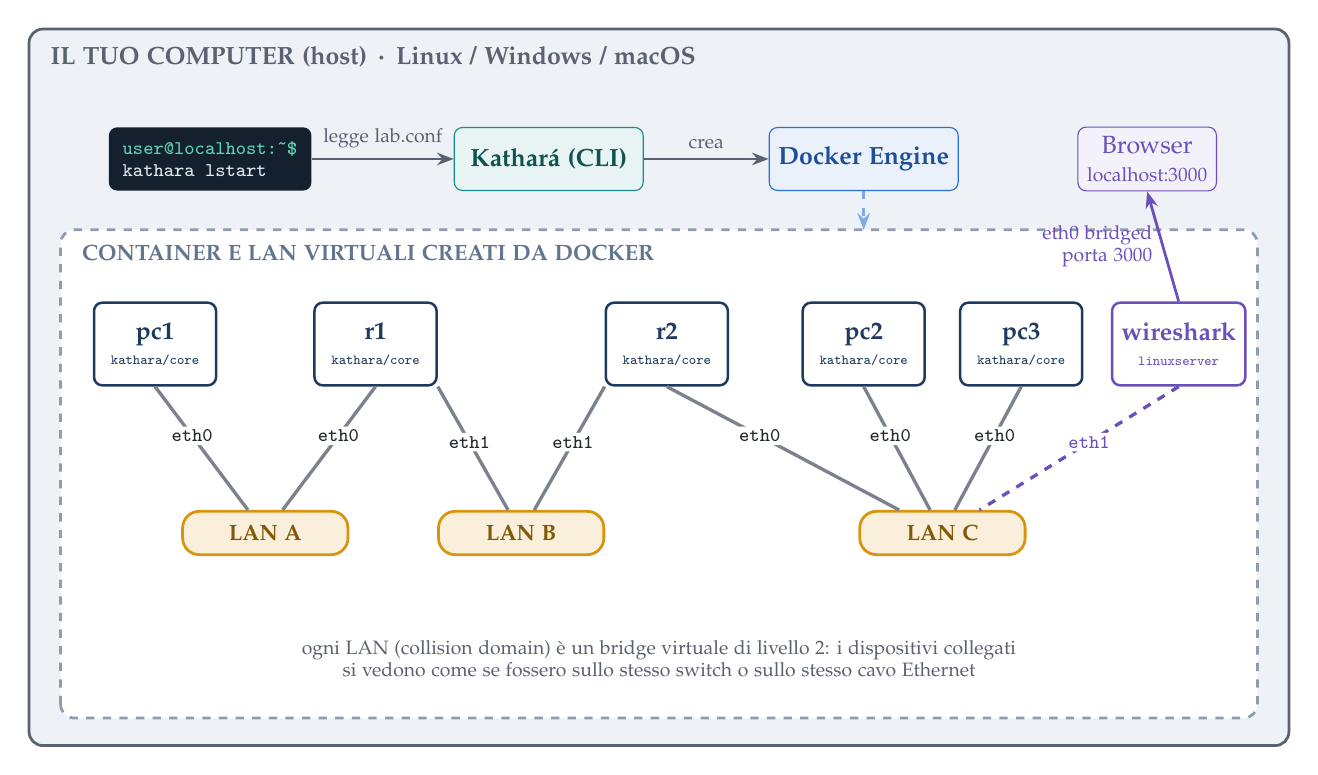
\begin{tikzpicture}[
  box/.style={rounded corners=5pt,line width=1pt},
  ctr/.style={rounded corners=3pt,draw=navy,fill=white,line width=.9pt,minimum width=1.55cm,minimum height=1.05cm,font=\headfont\bfseries\small,text=navy,align=center},
  br/.style={rounded corners=6pt,draw=ambra,fill=ambra!15,line width=1pt,minimum width=2.1cm,minimum height=.55cm,font=\headfont\bfseries\footnotesize,text=ambra!60!black},
  ar/.style={-{Stealth[length=6pt]},line width=1pt}]
  % host
  \draw[box,draw=grigio,fill=chiaro] (-1.0,-4.7) rectangle (15.0,4.4);
  \node[anchor=north west,font=\headfont\bfseries\small,text=grigio] at (-.85,4.3) {IL TUO COMPUTER (host) \,·\, Linux / Windows / macOS};
  % utente
  \node[rounded corners=3pt,fill=termbg,text=termfg,font=\ttfamily\scriptsize,align=left,inner sep=5pt] (term) at (1.3,2.75) {\color{termprompt}user@localhost:\textasciitilde\$\\kathara lstart};
  \node[rounded corners=3pt,draw=teal,fill=teal!10,font=\headfont\bfseries\small,text=teal!60!black,minimum width=2.4cm,minimum height=.8cm] (kat) at (5.6,2.75) {Kathará (CLI)};
  \node[rounded corners=3pt,draw=blu,fill=blu!10,font=\headfont\bfseries\small,text=blu!70!black,minimum width=2.4cm,minimum height=.8cm] (dock) at (9.6,2.75) {Docker Engine};
  \node[rounded corners=3pt,draw=viola,fill=viola!8,font=\headfont\small,text=viola,align=center,minimum height=.8cm] (brow) at (13.2,2.75) {Browser\\[-1pt]\scriptsize localhost:3000};
  \draw[ar,grigio] (term) -- node[above,font=\headfont\scriptsize]{legge lab.conf} (kat);
  \draw[ar,grigio] (kat) -- node[above,font=\headfont\scriptsize]{crea} (dock);
  % area container
  \draw[box,draw=navy!50,dashed,fill=white] (-.6,-4.35) rectangle (14.6,1.85);
  \node[anchor=north west,font=\headfont\bfseries\footnotesize,text=navy!70] at (-.45,1.78) {CONTAINER E LAN VIRTUALI CREATI DA DOCKER};
  \node[ctr] (pc1) at (.6,.4) {pc1\\[-2pt]\tiny\ttfamily kathara/core};
  \node[ctr] (r1) at (3.4,.4) {r1\\[-2pt]\tiny\ttfamily kathara/core};
  \node[ctr] (r2) at (7.1,.4) {r2\\[-2pt]\tiny\ttfamily kathara/core};
  \node[ctr] (pc2) at (9.6,.4) {pc2\\[-2pt]\tiny\ttfamily kathara/core};
  \node[ctr] (pc3) at (11.6,.4) {pc3\\[-2pt]\tiny\ttfamily kathara/core};
  \node[ctr,draw=viola,text=viola] (ws) at (13.6,.4) {wireshark\\[-2pt]\tiny\ttfamily linuxserver};
  \node[br] (A) at (2.0,-2.0) {LAN A};
  \node[br] (B) at (5.25,-2.0) {LAN B};
  \node[br] (C) at (10.6,-2.0) {LAN C};
  \draw[lnk] (pc1.south) -- node[lab,pos=.4]{eth0} (A);
  \draw[lnk] (r1.south) -- node[lab,pos=.4]{eth0} (A);
  \draw[lnk] (r1.south east) -- node[lab,pos=.45]{eth1} (B);
  \draw[lnk] (r2.south west) -- node[lab,pos=.45]{eth1} (B);
  \draw[lnk] (r2.south) -- node[lab,pos=.4]{eth0} (C);
  \draw[lnk] (pc2.south) -- node[lab,pos=.4]{eth0} (C);
  \draw[lnk] (pc3.south) -- node[lab,pos=.4]{eth0} (C);
  \draw[lnk,viola,dashed] (ws.south) -- node[lab,pos=.45,text=viola]{eth1} (C);
  \draw[ar,viola] (ws.north) -- node[left,font=\headfont\scriptsize,align=right,text=viola]{eth0 bridged\\porta 3000} (brow.south);
  \draw[ar,blu!60,dashed] (dock.south) -- (9.6,1.85);
  \node[font=\headfont\scriptsize,text=grigio,align=center] at (7.0,-3.6) {ogni LAN (collision domain) è un bridge virtuale di livello 2: i dispositivi collegati\\si vedono come se fossero sullo stesso switch o sullo stesso cavo Ethernet};
\end{tikzpicture}
\end{center}
\didascalia{Architettura del lab: Kathará legge la descrizione del laboratorio e chiede a Docker di creare un container per ogni dispositivo e una LAN virtuale per ogni collision domain. Il container wireshark ha anche un'interfaccia verso l'host, così l'interfaccia grafica si apre nel browser.}

\begin{tecnica}[Le tre idee chiave]
\begin{enumerate}
  \item \textbf{Dispositivo = container.} Un container è un processo isolato con il suo file system, i suoi processi e il suo \emph{stack di rete} (interfacce, indirizzi, tabella di routing, cache ARP). Per questo \texttt{r1} e \texttt{pc1} hanno tabelle di routing separate, anche se girano sullo stesso computer. I container condividono il kernel dell'host: sono molto più leggeri di una macchina virtuale.
  \item \textbf{Collision domain = LAN virtuale di livello 2.} Kathará realizza ogni collision domain con un bridge virtuale (tramite un plugin di rete di Docker). Tutto ciò che un dispositivo trasmette su quella LAN arriva agli altri dispositivi collegati alla stessa LAN, compresi i broadcast (come le richieste ARP). Due LAN diverse \textbf{non comunicano} tra loro, se non attraverso un router.
  \item \textbf{Interfacce numerate.} \texttt{device[0]} nel \texttt{lab.conf} diventa \texttt{eth0}, \texttt{device[1]} diventa \texttt{eth1}, e così via. Ogni interfaccia è come un cavo che va dal dispositivo alla LAN indicata.
\end{enumerate}
\end{tecnica}

\begin{attenzione}[Kathará non configura l'IP per te]
Kathará crea solo i «cavi» (livello 2). Gli indirizzi IP, le rotte e i servizi li configuri tu: a mano nel terminale del dispositivo, oppure nei file \texttt{.startup}, che Kathará esegue automaticamente all'avvio. Una configurazione scritta a mano nel terminale \textbf{si perde} quando il laboratorio viene chiuso.
\end{attenzione}

\subsection{Il ciclo di vita di un laboratorio}
\begin{center}
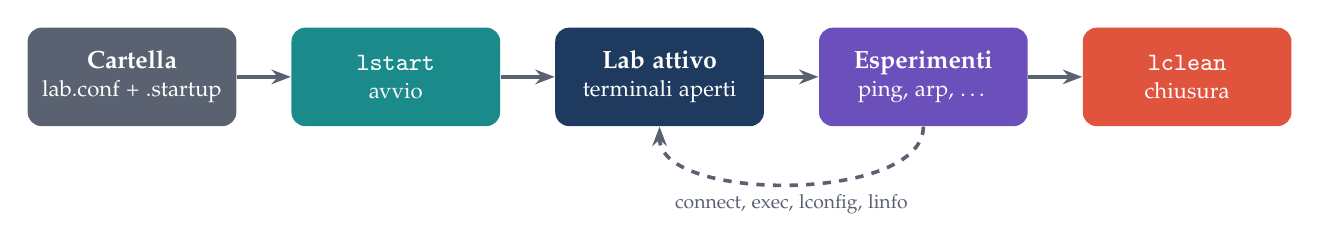
\begin{tikzpicture}[
  st/.style={rounded corners=5pt,minimum width=2.65cm,minimum height=1.25cm,font=\headfont\bfseries\small,align=center,text=white},
  ar/.style={-{Stealth[length=7pt]},line width=1.3pt,color=grigio}]
  \node[st,fill=grigio] (s1) at (0,0) {Cartella\\[-1pt]\footnotesize\mdseries lab.conf + .startup};
  \node[st,fill=teal] (s2) at (3.35,0) {\ttfamily lstart\\[-1pt]\footnotesize\headfont\mdseries avvio};
  \node[st,fill=navy] (s3) at (6.7,0) {Lab attivo\\[-1pt]\footnotesize\mdseries terminali aperti};
  \node[st,fill=viola] (s4) at (10.05,0) {Esperimenti\\[-1pt]\footnotesize\mdseries ping, arp, \dots};
  \node[st,fill=rosso] (s5) at (13.4,0) {\ttfamily lclean\\[-1pt]\footnotesize\headfont\mdseries chiusura};
  \draw[ar] (s1)--(s2); \draw[ar] (s2)--(s3); \draw[ar] (s3)--(s4); \draw[ar] (s4)--(s5);
  \draw[ar,dashed] (s4.south) .. controls (10.05,-1.6) and (6.7,-1.6) .. node[below,font=\headfont\scriptsize,text=grigio]{connect, exec, lconfig, linfo} (s3.south);
\end{tikzpicture}
\end{center}
\begin{enumerate}
  \item Ti sposti nella cartella del laboratorio (\cmd{cd}).
  \item \cmd{kathara lstart}: Kathará legge \texttt{lab.conf}, crea LAN e container, esegue i file \texttt{.startup} e apre un terminale per ogni dispositivo.
  \item Lavori nei terminali (\texttt{root@pc1:/\#}): verifichi la configurazione e fai gli esperimenti.
  \item Durante il lab puoi aprire altri terminali (\cmd{kathara connect}), lanciare comandi dall'host (\cmd{kathara exec}), collegare dispositivi ad altre LAN (\cmd{kathara lconfig}) e controllare lo stato (\cmd{kathara linfo}).
  \item \cmd{kathara lclean}: spegne e cancella container e LAN. La cartella con i file resta intatta: rilanciando \texttt{lstart} il lab riparte da zero, nello stato iniziale.
\end{enumerate}

\subsection{Dove si scrivono i comandi: host o dispositivo?}
È la confusione più comune all'inizio. Guarda sempre il \textbf{prompt}:
\begin{center}
\rowcolors{2}{chiaro}{white}
\begin{tabularx}{\linewidth}{l l Y}
\rowcolor{navy}\thd{Prompt} & \thd{Dove sei} & \thd{Comandi tipici}\\
\texttt{user@localhost:\textasciitilde\$} & sul tuo computer (host) & \texttt{kathara lstart}, \texttt{lclean}, \texttt{lconfig}, \texttt{connect}, \texttt{exec}\\
\texttt{root@pc1:/\#} & dentro il dispositivo \texttt{pc1} & \texttt{ip address}, \texttt{ip route}, \texttt{routel}, \texttt{ping}, \texttt{traceroute}, \texttt{arp}\\
\end{tabularx}
\end{center}
Dentro i dispositivi sei \texttt{root} (amministratore): puoi cambiare indirizzi e rotte senza \texttt{sudo}. I comandi \texttt{kathara} invece non esistono dentro i dispositivi.

\begin{mlbox}[Cartelle condivise]
Di default Kathará monta la sottocartella \texttt{shared/} del laboratorio come \texttt{/shared} dentro ogni dispositivo: è comodo per scambiare file (per esempio catture \texttt{.pcap}) tra host e dispositivi. Con l'opzione \texttt{--hosthome} di \texttt{lstart} si può montare anche la home dell'utente in \texttt{/hosthome} (disattivato di default).
\end{mlbox}

\begin{appunti}{Riepilogo del capitolo}
Dispositivo = container Docker con il proprio stack di rete. Collision domain = LAN virtuale L2 (bridge): broadcast inclusi, LAN diverse comunicano solo via router. \texttt{device[N]} $\to$ \texttt{ethN}. Kathará crea il livello 2; IP e rotte vanno nei \texttt{.startup} o si scrivono a mano (e si perdono con \texttt{lclean}). Prompt \texttt{\$} = host, \texttt{\#} = dispositivo.
\end{appunti}

\sezione{2}{Anatomia di un laboratorio}{lab.conf e file .startup}

\subsection{La cartella del laboratorio}
Un laboratorio Kathará è semplicemente una \textbf{cartella}. Il nome dei file è importante: Kathará riconosce i dispositivi dai nomi.
\begin{center}
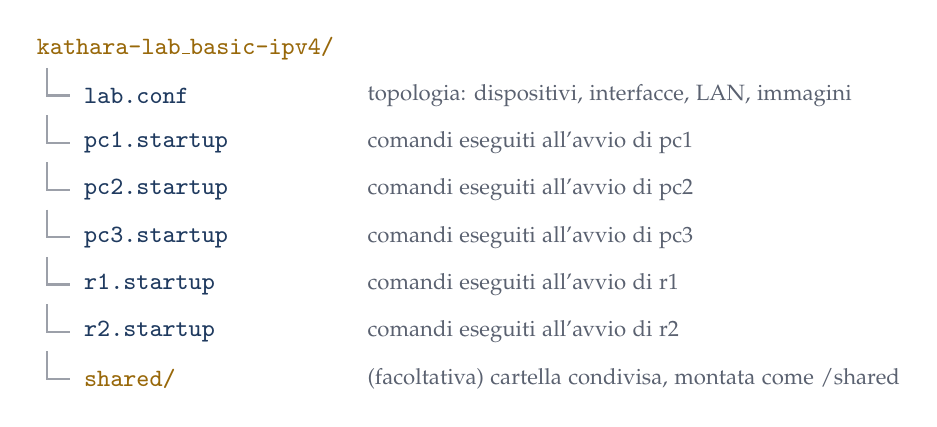
\begin{tikzpicture}[
  f/.style={anchor=west,font=\ttfamily\small,text=navy},
  d/.style={anchor=west,font=\ttfamily\small\bfseries,text=ambra!70!black},
  c/.style={anchor=west,font=\headfont\footnotesize,text=grigio}]
  \node[d] (root) at (0,0) {kathara-lab\_basic-ipv4/};
  \draw[grigio!60,line width=.8pt] (.25,-0.25) |- (.55,-0.6);
  \node[f] at (.6,-0.6) {lab.conf};
  \node[c] at (4.2,-0.6) {topologia: dispositivi, interfacce, LAN, immagini};
  \draw[grigio!60,line width=.8pt] (.25,-0.85) |- (.55,-1.2);
  \node[f] at (.6,-1.2) {pc1.startup};
  \node[c] at (4.2,-1.2) {comandi eseguiti all'avvio di pc1};
  \draw[grigio!60,line width=.8pt] (.25,-1.45) |- (.55,-1.8);
  \node[f] at (.6,-1.8) {pc2.startup};
  \node[c] at (4.2,-1.8) {comandi eseguiti all'avvio di pc2};
  \draw[grigio!60,line width=.8pt] (.25,-2.05) |- (.55,-2.4);
  \node[f] at (.6,-2.4) {pc3.startup};
  \node[c] at (4.2,-2.4) {comandi eseguiti all'avvio di pc3};
  \draw[grigio!60,line width=.8pt] (.25,-2.65) |- (.55,-3.0);
  \node[f] at (.6,-3.0) {r1.startup};
  \node[c] at (4.2,-3.0) {comandi eseguiti all'avvio di r1};
  \draw[grigio!60,line width=.8pt] (.25,-3.25) |- (.55,-3.6);
  \node[f] at (.6,-3.6) {r2.startup};
  \node[c] at (4.2,-3.6) {comandi eseguiti all'avvio di r2};
  \draw[grigio!60,line width=.8pt] (.25,-3.85) |- (.55,-4.2);
  \node[d] at (.6,-4.2) {shared/};
  \node[c] at (4.2,-4.2) {(facoltativa) cartella condivisa, montata come /shared};
\end{tikzpicture}
\end{center}
\begin{tecnica}[Regole dei nomi]
\begin{itemize}
  \item Un dispositivo esiste se compare nel \texttt{lab.conf} (o se ha una cartella o un file \texttt{.startup} con il suo nome).
  \item \texttt{pc1.startup} è uno script di shell eseguito \textbf{dentro} \texttt{pc1} appena il container parte.
  \item Una eventuale cartella \texttt{pc1/} viene copiata nel file system di \texttt{pc1} (per esempio \texttt{pc1/etc/...} finisce in \texttt{/etc/...}): serve nei lab con servizi come DNS o web server. In questo lab non c'è.
\end{itemize}
\end{tecnica}

\subsection{Il file lab.conf}
La sintassi è una sequenza di assegnamenti \texttt{dispositivo[argomento]=valore}. Le righe che iniziano con \texttt{\#} sono commenti.
\begin{filecfg}{lab.conf}
°# --- router r1: eth0 su A, eth1 su B, MAC scelti a mano ---°
§r1[0]§="A/00:00:00:00:00:a1"
§r1[1]§="B/00:00:00:00:00:b1"
r1[image]="kathara/core"
r1[ipv6]="false"

§r2[0]§="C/00:00:00:00:00:c1"
§r2[1]§="B/00:00:00:00:00:b2"
r2[image]="kathara/core"
r2[ipv6]="false"

§pc1[0]§="A/00:00:00:00:00:01"
pc1[image]="kathara/core"
pc1[ipv6]="false"

§pc2[0]§="C/00:00:00:00:00:02"
pc2[image]="kathara/core"
pc2[ipv6]="false"

§pc3[0]§="C/00:00:00:00:00:03"
pc3[image]="kathara/core"
pc3[ipv6]="false"

°# --- dispositivo speciale per catturare il traffico ---°
wireshark[bridged]=true
wireshark[port]="3000:3000"
wireshark[image]="lscr.io/linuxserver/wireshark"
wireshark[num_terms]=0
\end{filecfg}

\subsubsection{Come si legge una riga di interfaccia}
\begin{center}
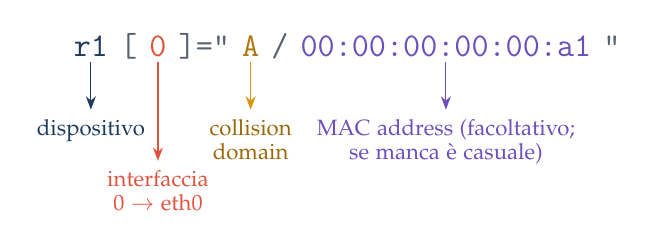
\begin{tikzpicture}[part/.style={font=\ttfamily\large,inner sep=2pt},
  ex/.style={font=\headfont\footnotesize,align=center,text=grigio}]
  \node[part,text=navy] (a) at (0,0) {r1};
  \node[part,text=grigio,anchor=west] (b) at (a.east) {[};
  \node[part,text=rosso,anchor=west] (c) at (b.east) {0};
  \node[part,text=grigio,anchor=west] (d) at (c.east) {]="};
  \node[part,text=ambra!80!black,anchor=west] (e) at (d.east) {A};
  \node[part,text=grigio,anchor=west] (f) at (e.east) {/};
  \node[part,text=viola,anchor=west] (g) at (f.east) {00:00:00:00:00:a1};
  \node[part,text=grigio,anchor=west] (h) at (g.east) {"};
  \draw[navy,-{Stealth}] (a.south) -- ++(0,-.6) node[below,ex,text=navy]{dispositivo};
  \draw[rosso,-{Stealth}] (c.south) -- ++(0,-1.25) node[below,ex,text=rosso]{interfaccia\\[-1pt]0 $\to$ eth0};
  \draw[ambra,-{Stealth}] (e.south) -- ++(0,-.6) node[below,ex,text=ambra!70!black]{collision\\[-1pt]domain};
  \draw[viola,-{Stealth}] (g.south) -- ++(0,-.6) node[below,ex,text=viola]{MAC address (facoltativo;\\[-1pt]se manca è casuale)};
\end{tikzpicture}
\end{center}
«Collega l'interfaccia \texttt{eth0} di \texttt{r1} alla LAN \texttt{A} e dagli il MAC \texttt{00:00:00:00:00:a1}.»

\subsubsection{Le opzioni usate nel lab}
\begin{center}
\rowcolors{2}{chiaro}{white}
\begin{tabularx}{\linewidth}{>{\ttfamily}l Y}
\rowcolor{navy}\thd{Opzione} & \thd{Significato}\\
image="kathara/core" & immagine Docker del dispositivo: una Debian con gli strumenti di rete (\texttt{ip}, \texttt{ping}, \texttt{traceroute}, \texttt{arp}, \dots)\\
ipv6="false" & disattiva IPv6: le catture restano pulite, senza i messaggi IPv6 automatici\\
bridged=true & aggiunge un'interfaccia collegata alla rete dell'host tramite NAT (sarà \texttt{eth0})\\
port="3000:3000" & inoltra la porta 3000 dell'host alla porta 3000 del container (\texttt{HOST:GUEST})\\
num\_terms=0 & numero di terminali da aprire per il dispositivo: 0 = nessuno\\
\end{tabularx}
\end{center}
Altre opzioni utili: \texttt{mem} e \texttt{cpus} (limiti di risorse), \texttt{exec} (comando all'avvio), \texttt{sysctl} (parametri del kernel di rete), \texttt{env} (variabili d'ambiente), \texttt{shell} (shell usata da \texttt{connect}). Si possono anche aggiungere metadati come \texttt{LAB\_NAME}, \texttt{LAB\_DESCRIPTION}, \texttt{LAB\_AUTHOR}, mostrati all'avvio.

\begin{mlbox}[Perché MAC «leggibili»]
Di norma Kathará assegna MAC casuali. Qui sono forzati: \texttt{01}, \texttt{02}, \texttt{03} per i pc; \texttt{a1}, \texttt{b1}, \texttt{b2}, \texttt{c1} per le interfacce dei router (la lettera indica la LAN). Così nelle catture Wireshark e nella cache ARP si capisce a colpo d'occhio chi sta parlando.
\end{mlbox}

\subsection{Il dispositivo wireshark}
\begin{intuizione}
È un container speciale che contiene Wireshark con un'interfaccia grafica raggiungibile \textbf{dal browser}. All'avvio è collegato solo all'host (\texttt{bridged}, interfaccia \texttt{eth0}); quando vuoi osservare una LAN, lo «colleghi» con \texttt{kathara lconfig}, come se attaccassi un cavo dal tuo PC di analisi allo switch di quella LAN. Non apre terminali (\texttt{num\_terms=0}): si usa solo dal browser su \texttt{localhost:3000}.
\end{intuizione}
\begin{attenzione}[Quale interfaccia sniffare]
Le interfacce aggiunte con \texttt{lconfig} sono numerate \textbf{in ordine dopo l'ultima esistente}. Nel lab: \texttt{eth0} = bridged (verso l'host), la prima LAN aggiunta (C) diventa \texttt{eth1}, la seconda (B) diventa \texttt{eth2}. Per questo le slide dicono di sniffare \texttt{eth1} su C e \texttt{eth2} su B.
\end{attenzione}

\subsection{I file .startup}
Sono script di shell: ogni riga è un comando eseguito dentro il dispositivo all'avvio, come se lo scrivessi tu nel suo terminale.

\begin{filecfg}{pc1.startup}
ip address add 195.11.14.5/24 dev eth0
ip route add default via 195.11.14.1
\end{filecfg}
\begin{filecfg}{pc2.startup}
ip address add 200.1.1.7/24 dev eth0
ip route add default via 200.1.1.1 dev eth0
\end{filecfg}
\begin{filecfg}{pc3.startup}
ip address add 200.1.1.3/24 dev eth0
ip route add default via 200.1.1.1 dev eth0
\end{filecfg}
\begin{tecnica}[Cosa fanno, riga per riga (host)]
\begin{enumerate}
  \item \inl{ip address add 195.11.14.5/24 dev eth0}: assegna a \texttt{eth0} l'indirizzo \texttt{195.11.14.5} con maschera \texttt{/24} (255.255.255.0). Effetto collaterale importante: il kernel aggiunge da solo la rotta verso la rete \texttt{195.11.14.0/24}, che diventa \textbf{direttamente connessa}.
  \item \inl{ip route add default via 195.11.14.1}: imposta il \textbf{default gateway}. Tutto ciò che non è destinato alla propria LAN va consegnato a \texttt{195.11.14.1}, cioè a \texttt{r1}. In pc2 e pc3 c'è anche \texttt{dev eth0}, che indica esplicitamente l'interfaccia di uscita; in pc1 manca perché il kernel la deduce da solo (il gateway sta su una rete di \texttt{eth0}).
\end{enumerate}
\end{tecnica}

\begin{filecfg}{r1.startup}
ip address add 195.11.14.1/24 dev eth0    °# LAN A: rete direttamente connessa°
ip address add 100.0.0.9/30 dev eth1      °# LAN B: rete direttamente connessa°
ip route add 200.1.1.0/24 via 100.0.0.10 dev eth1   °# LAN C: rotta statica°
\end{filecfg}
\begin{filecfg}{r2.startup  (ricostruito)}
ip address add 200.1.1.1/24 dev eth0
ip address add 100.0.0.10/30 dev eth1
ip route add 195.11.14.0/24 via 100.0.0.9 dev eth1
\end{filecfg}
\begin{tecnica}[Cosa fanno (router)]
\begin{itemize}
  \item Le prime due righe danno un indirizzo a ciascuna interfaccia: le reti A e B (per r1) diventano \textbf{direttamente connesse} e non serve scrivere rotte per raggiungerle.
  \item La terza riga aggiunge una \textbf{rotta statica} verso l'unica LAN che il router non vede direttamente: per r1 è C (\texttt{200.1.1.0/24}), raggiungibile consegnando i pacchetti a r2 (\texttt{100.0.0.10}) attraverso \texttt{eth1}.
  \item Le slide mostrano solo \texttt{r1.startup} e dicono «configurazione analoga per r2»: il file di r2 qui sopra è ricostruito dalla topologia ed è coerente con il piano di indirizzamento.
\end{itemize}
\end{tecnica}
\begin{attenzione}[Il forwarding]
Un router Linux inoltra i pacchetti tra le sue interfacce solo se è attivo il parametro \texttt{net.ipv4.ip\_forward}. Kathará lo attiva di default all'avvio dei dispositivi, ed è per questo che \texttt{r1} e \texttt{r2} funzionano da router senza comandi aggiuntivi (e, in linea di principio, anche un pc inoltrerebbe pacchetti se ne ricevesse da inoltrare). Se in un tuo lab un «router» non inoltra, controlla con \inl{sysctl net.ipv4.ip\_forward} (deve valere 1).
\end{attenzione}

\begin{appunti}{Riepilogo del capitolo}
Lab = cartella con \texttt{lab.conf} + \texttt{<dev>.startup} (+ \texttt{shared/}, cartelle per dispositivo). \texttt{dev[N]="CD/MAC"} collega \texttt{ethN} alla LAN \texttt{CD}. Opzioni: \texttt{image}, \texttt{ipv6}, \texttt{bridged}, \texttt{port}, \texttt{num\_terms}. Host: indirizzo + default gateway. Router: un indirizzo per interfaccia (reti dirette) + rotta statica verso la LAN remota. wireshark: \texttt{eth0} bridged, poi \texttt{eth1}, \texttt{eth2}\dots{} nell'ordine di \texttt{lconfig}.
\end{appunti}

\sezione{3}{La rete del lab basic-ipv4}{topologia e indirizzi}

\subsection{Chi c'è nella rete}
Due router (\texttt{r1}, \texttt{r2}) e tre host (\texttt{pc1}, \texttt{pc2}, \texttt{pc3}) collegati da tre LAN (collision domain \texttt{A}, \texttt{B}, \texttt{C}). Nel laboratorio imparerai a:
\begin{itemize}
  \item assegnare un indirizzo IPv4 e una netmask a un'interfaccia;
  \item impostare il default gateway di un host;
  \item impostare la tabella di routing di un router;
  \item usare \texttt{ping} e \texttt{traceroute} e osservare il comportamento di ARP.
\end{itemize}

\subsection{La topologia completa}
\begin{center}
\topologia{1}{1}{1}
\end{center}
\didascalia{In giallo i collision domain (LAN), in verde le reti IP, in rosso l'ultimo ottetto dell'indirizzo di ogni interfaccia, in viola i MAC address. Per esempio \texttt{r1} ha \texttt{eth0} = \texttt{195.11.14.1} (MAC \texttt{00:..:a1}) su A ed \texttt{eth1} = \texttt{100.0.0.9} (MAC \texttt{00:..:b1}) su B.}

\begin{center}
\rowcolors{2}{chiaro}{white}
\begin{tabular}{l l c l l l}
\rowcolor{navy}\thd{Dispositivo} & \thd{Interfaccia} & \thd{LAN} & \thd{Indirizzo IPv4} & \thd{MAC} & \thd{Default gateway}\\
pc1 & eth0 & A & 195.11.14.5/24 & 00:00:00:00:00:01 & 195.11.14.1 (r1)\\
pc2 & eth0 & C & 200.1.1.7/24 & 00:00:00:00:00:02 & 200.1.1.1 (r2)\\
pc3 & eth0 & C & 200.1.1.3/24 & 00:00:00:00:00:03 & 200.1.1.1 (r2)\\
r1 & eth0 & A & 195.11.14.1/24 & 00:00:00:00:00:a1 & —\\
r1 & eth1 & B & 100.0.0.9/30 & 00:00:00:00:00:b1 & —\\
r2 & eth0 & C & 200.1.1.1/24 & 00:00:00:00:00:c1 & —\\
r2 & eth1 & B & 100.0.0.10/30 & 00:00:00:00:00:b2 & —\\
\end{tabular}
\end{center}

\subsection{Capire le maschere: /24 e /30}
\begin{tecnica}[Notazione CIDR]
Il numero dopo la barra dice quanti bit (da sinistra) identificano la \textbf{rete}; i restanti identificano l'\textbf{host}.
\begin{itemize}
  \item \texttt{/24} = maschera \texttt{255.255.255.0}: 8 bit di host, $2^8=256$ indirizzi. Il primo (\texttt{.0}) è l'indirizzo di rete, l'ultimo (\texttt{.255}) il broadcast: restano \textbf{254} indirizzi utilizzabili.
  \item \texttt{/30} = maschera \texttt{255.255.255.252}: 2 bit di host, 4 indirizzi. Restano \textbf{2} indirizzi utilizzabili: è la rete perfetta per un collegamento punto-punto tra due router.
\end{itemize}
\end{tecnica}
\begin{esempio}[La LAN B: 100.0.0.8/30]
\begin{center}
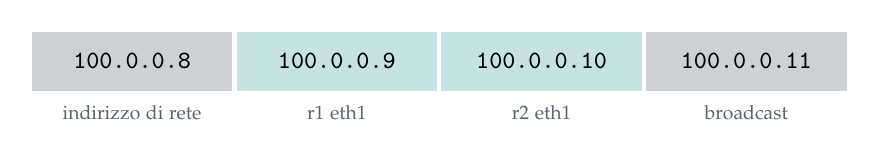
\begin{tikzpicture}[c/.style={minimum width=2.6cm,minimum height=.8cm,font=\ttfamily\small,draw=white,line width=1.5pt}]
  \node[c,fill=grigio!30] at (0,0) {100.0.0.8};
  \node[c,fill=teal!25] at (2.6,0) {100.0.0.9};
  \node[c,fill=teal!25] at (5.2,0) {100.0.0.10};
  \node[c,fill=grigio!30] at (7.8,0) {100.0.0.11};
  \foreach \x/\t in {0/indirizzo di rete,2.6/r1 eth1,5.2/r2 eth1,7.8/broadcast}{\node[font=\headfont\scriptsize,text=grigio] at (\x,-.65) {\t};}
\end{tikzpicture}
\end{center}
In binario l'ultimo ottetto è \texttt{000010\textbf{00}}…\texttt{000010\textbf{11}}: i primi 6 bit sono fissi (parte di rete), gli ultimi 2 variano. Ecco perché nella tabella di \texttt{r1} comparirà \texttt{100.0.0.11} come indirizzo di broadcast della LAN B.
\end{esempio}

\subsection{Chi sa cosa: la logica del routing}
\begin{intuizione}
Ogni dispositivo conosce «da solo» solo le reti a cui è attaccato direttamente. Per tutto il resto serve un'indicazione esplicita.
\begin{itemize}
  \item \textbf{Gli host} sanno raggiungere la propria LAN; per tutto il resto usano il \textbf{default gateway} («se non sai dove mandarlo, dallo al router»).
  \item \textbf{r1} conosce A e B (direttamente connesse); per C ha una \textbf{rotta statica} via r2.
  \item \textbf{r2} conosce B e C; per A ha una rotta statica via r1.
\end{itemize}
Con queste informazioni ogni host può raggiungere ogni altro host, in entrambe le direzioni.
\end{intuizione}
\begin{center}
\rowcolors{2}{chiaro}{white}
\begin{tabular}{l c c c}
\rowcolor{navy}\thd{} & \thd{LAN A (195.11.14.0/24)} & \thd{LAN B (100.0.0.8/30)} & \thd{LAN C (200.1.1.0/24)}\\
pc1 & diretta & default via r1 & default via r1\\
pc2, pc3 & default via r2 & default via r2 & diretta\\
r1 & diretta (eth0) & diretta (eth1) & \textbf{statica} via 100.0.0.10\\
r2 & \textbf{statica} via 100.0.0.9 & diretta (eth1) & diretta (eth0)\\
\end{tabular}
\end{center}

\begin{attenzione}[Il ritorno conta quanto l'andata]
Un ping funziona solo se esiste la rotta \emph{anche per la risposta}. Se togli la rotta statica da r2, pc1 riesce ancora a mandare la richiesta a pc2 (grazie a r1), ma la risposta di pc2 si ferma su r2, che non sa dove sia \texttt{195.11.14.0/24}. È uno degli errori più frequenti nei laboratori di routing.
\end{attenzione}

\begin{appunti}{Riepilogo del capitolo}
3 LAN: A = 195.11.14.0/24 (pc1 .5, r1 .1); B = 100.0.0.8/30 (r1 .9, r2 .10, broadcast .11); C = 200.1.1.0/24 (pc2 .7, pc3 .3, r2 .1). Host: rete diretta + default gateway. Router: due reti dirette + una rotta statica verso la LAN remota. Le rotte servono in entrambe le direzioni.
\end{appunti}

\sezione{4}{I comandi di Kathará}{si usano sull'host}

Tutti questi comandi si scrivono nel terminale del \textbf{tuo computer} (prompt \texttt{\$}), di solito dopo essersi spostati nella cartella del laboratorio. Hanno tutti la forma \texttt{kathara <sottocomando> [opzioni]}; \sint{kathara <sottocomando> -h} mostra l'aiuto. I comandi che iniziano con \textbf{l} (\emph{lab}) agiscono su un intero laboratorio; quelli con \textbf{v} su un singolo dispositivo creato a mano.

\begin{center}
\rowcolors{2}{chiaro}{white}
\begin{tabularx}{\linewidth}{>{\ttfamily\bfseries\color{navy}}l Y >{\ttfamily\small}l}
\rowcolor{navy}\thd{Comando} & \thd{A cosa serve} & \thd{Esempio tipico}\\
lstart & avvia il laboratorio della cartella & kathara lstart\\
lclean & spegne e cancella il laboratorio & kathara lclean\\
lrestart & riavvia (lclean + lstart) & kathara lrestart\\
connect & apre un terminale su un dispositivo & kathara connect pc1\\
exec & esegue un comando su un dispositivo & kathara exec pc3 "arp -n"\\
lconfig & collega/scollega un dispositivo a una LAN & kathara lconfig -n wireshark --add C\\
linfo & mostra stato e topologia del lab & kathara linfo\\
list & elenca tutti i dispositivi attivi & kathara list\\
wipe & spegne \emph{tutti} i dispositivi Kathará & kathara wipe\\
check & controlla l'installazione & kathara check\\
\end{tabularx}
\end{center}

% ---------------- LSTART ----------------
\begin{scheda}{kathara lstart}
\campo{Sintassi}
\sint{kathara lstart [-d CARTELLA] [--noterminals | --terminals] [--print] [-l] [-o OPZIONE ...] [DISPOSITIVO ...]}
\campo{Cosa fa}
Avvia il laboratorio: legge \texttt{lab.conf}, crea le LAN (collision domain) e un container per ogni dispositivo, esegue i file \texttt{.startup} e (salvo diversa impostazione) apre un terminale per ogni dispositivo.
\campo{Opzioni principali}
\begin{tabularx}{\linewidth}{>{\ttfamily\small}l Y}
-d CARTELLA & avvia il lab che sta in un'altra cartella (default: quella corrente)\\
--noterminals & non apre le finestre di terminale (poi ci si collega con \texttt{connect})\\
--terminals & apre comunque i terminali\\
--print & controlla il \texttt{lab.conf} senza avviare nulla (prova a secco)\\
-l, --list & mostra le informazioni sui dispositivi dopo l'avvio\\
-o "opt=valore" & applica un'opzione a tutti i dispositivi (es. \texttt{-o "mem=64m"})\\
DISPOSITIVO ... & avvia solo i dispositivi elencati\\
--exclude D ... & avvia tutto tranne i dispositivi elencati\\
\end{tabularx}
\campo{Esempio}
\begin{terminale}{host}
§user@localhost:~$§ cd kathara-lab_basic-ipv4
§user@localhost:~/kathara-lab_basic-ipv4$§ kathara lstart
°... Kathará crea le LAN A, B, C e i dispositivi r1, r2, pc1, pc2, pc3, wireshark°
°... si aprono 5 terminali (wireshark ha num_terms=0)°
\end{terminale}
\end{scheda}
\begin{attenzione}[Errori tipici all'avvio]
\begin{itemize}
  \item \textbf{Non sei nella cartella giusta}: Kathará non trova \texttt{lab.conf}. Usa \texttt{cd} oppure \texttt{-d}.
  \item \textbf{Il lab è già attivo}: prima \texttt{kathara lclean}, poi di nuovo \texttt{lstart}.
  \item \textbf{Docker non è avviato}: Kathará non riesce a creare i container. Avvia Docker (Docker Desktop su Windows/macOS) e riprova; \texttt{kathara check} aiuta a diagnosticare.
  \item La prima volta l'avvio è lento: Docker scarica le immagini (\texttt{kathara/core}, quella di Wireshark).
\end{itemize}
\end{attenzione}

% ---------------- LCLEAN ----------------
\begin{scheda}{kathara lclean}
\campo{Sintassi}
\sint{kathara lclean [-d CARTELLA] [--exclude DISPOSITIVO ...] [DISPOSITIVO ...]}
\campo{Cosa fa}
Spegne il laboratorio: chiude i terminali, ferma e cancella i container e le LAN. I file della cartella (\texttt{lab.conf}, \texttt{.startup}) restano intatti, mentre tutto ciò che hai configurato a mano nei terminali va perso.
\campo{Esempi}
\begin{terminale}{host}
§user@localhost:~/kathara-lab_basic-ipv4$§ kathara lclean          °# spegne tutto il lab°
§user@localhost:~/kathara-lab_basic-ipv4$§ kathara lclean pc1 pc2  °# spegne solo pc1 e pc2°
\end{terminale}
\end{scheda}

\begin{scheda}{kathara lrestart}
\campo{Cosa fa}
Equivale a \texttt{lclean} seguito da \texttt{lstart}: riporta il laboratorio allo stato iniziale. Utile quando hai «rotto» la configurazione durante un esercizio e vuoi ricominciare. Accetta le stesse opzioni principali di \texttt{lstart} (\texttt{-d}, \texttt{--noterminals}, \dots).
\end{scheda}

% ---------------- CONNECT ----------------
\begin{scheda}{kathara connect}
\campo{Sintassi}
\sint{kathara connect [-d CARTELLA] [-l] DISPOSITIVO}
\campo{Cosa fa}
Apre una shell \textbf{dentro} un dispositivo del laboratorio, nel terminale in cui ti trovi. Serve se hai chiuso per sbaglio la finestra di un dispositivo, se hai avviato il lab con \texttt{--noterminals}, o se vuoi un secondo terminale sullo stesso dispositivo (per esempio uno per \texttt{ping} e uno per guardare la cache ARP).
\campo{Opzioni}
\begin{tabularx}{\linewidth}{>{\ttfamily\small}l Y}
-l, --logs & mostra prima i log di avvio del dispositivo (utile per vedere errori nel \texttt{.startup})\\
--command SHELL & usa una shell diversa da quella predefinita\\
\end{tabularx}
\campo{Esempio}
\begin{terminale}{host}
§user@localhost:~/kathara-lab_basic-ipv4$§ kathara connect pc3
§root@pc3:/#§ arp -n
§root@pc3:/#§ exit      °# torna al terminale dell'host°
\end{terminale}
\end{scheda}

% ---------------- EXEC ----------------
\begin{scheda}{kathara exec}
\campo{Sintassi}
\sint{kathara exec [-d CARTELLA] [--no-stdout] [--no-stderr] [--wait] DISPOSITIVO COMANDO}
\campo{Cosa fa}
Esegue \textbf{un solo comando} dentro un dispositivo e ne stampa l'output sull'host, senza aprire una shell interattiva. Comodo per controlli rapidi o per script che interrogano più dispositivi. Il comando, se contiene spazi, va tra virgolette.
\campo{Esempi}
\begin{terminale}{host}
§user@localhost:~/kathara-lab_basic-ipv4$§ kathara exec r1 "ip route"
100.0.0.8/30 dev eth1 proto kernel scope link src 100.0.0.9
195.11.14.0/24 dev eth0 proto kernel scope link src 195.11.14.1
200.1.1.0/24 via 100.0.0.10 dev eth1
§user@localhost:~/kathara-lab_basic-ipv4$§ kathara exec pc3 "ping -c 2 200.1.1.7"
\end{terminale}
\end{scheda}

% ---------------- LCONFIG ----------------
\begin{scheda}{kathara lconfig}
\campo{Sintassi}
\sint{kathara lconfig [-d CARTELLA] -n DISPOSITIVO (--add LAN[/MAC] ... | --rm LAN ...)}
\campo{Cosa fa}
Modifica \textbf{a caldo} (con il lab acceso) i collegamenti di un dispositivo: \texttt{--add} aggiunge una nuova interfaccia collegata alla LAN indicata, \texttt{--rm} la toglie. È l'equivalente di attaccare o staccare un cavo. Le nuove interfacce prendono il numero successivo all'ultima esistente.
\campo{Opzioni}
\begin{tabularx}{\linewidth}{>{\ttfamily\small}l Y}
-n DISPOSITIVO & dispositivo da modificare (obbligatorio)\\
--add LAN[/MAC] & collega il dispositivo a una o più LAN (MAC facoltativo)\\
--rm LAN & scollega il dispositivo dalla LAN e rimuove l'interfaccia\\
\end{tabularx}
\campo{Esempi del lab}
\begin{terminale}{host}
§user@localhost:~/kathara-lab_basic-ipv4$§ kathara lconfig -n wireshark --add C
°# wireshark ottiene eth1 collegata alla LAN C°
§user@localhost:~/kathara-lab_basic-ipv4$§ kathara lconfig -n wireshark --add B
°# wireshark ottiene eth2 collegata alla LAN B°
§user@localhost:~/kathara-lab_basic-ipv4$§ kathara lconfig -n wireshark --rm C
°# stacca wireshark dalla LAN C°
\end{terminale}
\end{scheda}
\begin{center}
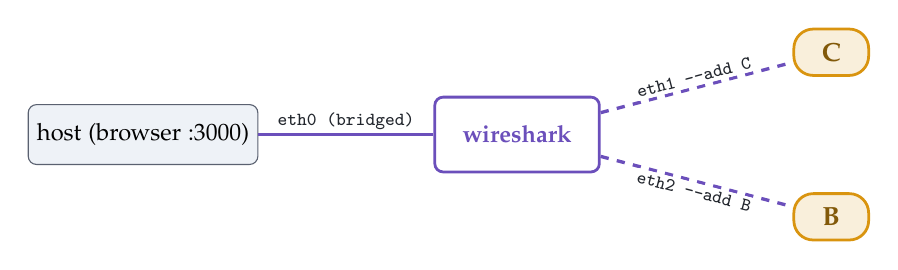
\begin{tikzpicture}[scale=.95,transform shape]
  \node[dev,draw=viola,text=viola,minimum width=2.2cm,minimum height=1cm] (ws) at (0,0) {wireshark};
  \node[rounded corners=3pt,draw=grigio,fill=chiaro,font=\headfont\small,minimum height=.8cm] (h) at (-5,0) {host (browser :3000)};
  \node[cd] (C) at (4.2,1.1) {C};
  \node[cd] (B) at (4.2,-1.1) {B};
  \draw[lnk,viola] (ws) -- node[lab,above]{eth0 (bridged)} (h);
  \draw[lnk,viola,dashed] (ws) -- node[lab,sloped,above]{eth1 \texttt{--add C}} (C);
  \draw[lnk,viola,dashed] (ws) -- node[lab,sloped,below]{eth2 \texttt{--add B}} (B);
\end{tikzpicture}
\end{center}
\didascalia{Il container wireshark dopo i due \texttt{lconfig}: l'ordine delle aggiunte decide il nome dell'interfaccia da sniffare.}

% ---------------- LINFO ----------------
\begin{scheda}{kathara linfo}
\campo{Sintassi}
\sint{kathara linfo [-d CARTELLA] [-w] [-c] [-n DISPOSITIVO | -t]}
\campo{Cosa fa}
Mostra lo stato del laboratorio: per ogni dispositivo nome, stato, uso di CPU e memoria, traffico di rete.
\campo{Opzioni}
\begin{tabularx}{\linewidth}{>{\ttfamily\small}l Y}
-w, --watch & aggiorna i dati in tempo reale (esci con \texttt{Ctrl+C})\\
-c, --conf & mostra solo le informazioni statiche del \texttt{lab.conf} (descrizione, numero di dispositivi e reti), anche a lab spento\\
-t, --topology & mostra quali dispositivi sono collegati a ciascun collision domain\\
-n DISPOSITIVO & limita le informazioni a un dispositivo\\
\end{tabularx}
\end{scheda}

\begin{scheda}{kathara list \quad·\quad kathara wipe \quad·\quad kathara check}
\campo{kathara list}
Elenca \textbf{tutti} i dispositivi Kathará in esecuzione per l'utente, di qualunque laboratorio. Utile se non ricordi quali lab hai lasciato accesi.
\campo{kathara wipe}
Spegne \textbf{tutti} i dispositivi e le LAN Kathará dell'utente, di qualunque laboratorio (chiede conferma; \texttt{-f} la salta). È il «pulsante di emergenza» se qualcosa è rimasto appeso. Con \texttt{-s} invece ripristina solo le impostazioni di Kathará.
\campo{kathara check}
Verifica l'ambiente (versione di Kathará, Docker raggiungibile, prova di avvio): il primo comando da lanciare se l'installazione non funziona.
\end{scheda}

\begin{mlbox}[Dispositivi singoli: vstart, vclean, vconfig]
Oltre ai laboratori, Kathará può creare un dispositivo isolato «al volo»: \sint{kathara vstart -n pc1 --eth 0:A} crea \texttt{pc1} con \texttt{eth0} sulla LAN \texttt{A}; \sint{kathara vclean -n pc1} lo elimina; \texttt{vconfig} ne modifica le interfacce. Con questi dispositivi \texttt{connect} ed \texttt{exec} vogliono l'opzione \texttt{-v}. Per il lab basic-ipv4 non servono: è tutto descritto nel \texttt{lab.conf}.
\end{mlbox}

\begin{appunti}{Riepilogo del capitolo}
\texttt{lstart} avvia, \texttt{lclean} spegne (e cancella le modifiche a mano), \texttt{lrestart} = lclean + lstart. \texttt{connect D} = shell su D; \texttt{exec D "cmd"} = un comando su D. \texttt{lconfig -n D --add/--rm LAN} = attacca/stacca un cavo (interfacce numerate in ordine). \texttt{linfo} = stato (\texttt{-t} topologia, \texttt{-w} live). \texttt{list} = tutti i dispositivi attivi; \texttt{wipe} = spegne tutto; \texttt{check} = diagnostica.
\end{appunti}

\sezione{5}{I comandi Linux nei dispositivi}{si usano nei terminali dei device}

Questi comandi si scrivono nei terminali dei dispositivi (prompt \texttt{root@pc1:/\#}). Sono i normali comandi di rete di Linux: funzionano allo stesso modo su un server reale.

\begin{center}
\rowcolors{2}{chiaro}{white}
\begin{tabularx}{\linewidth}{>{\ttfamily\bfseries\color{navy}}l Y >{\ttfamily\small}l}
\rowcolor{navy}\thd{Comando} & \thd{A cosa serve} & \thd{Abbreviazione}\\
ip address & mostra/assegna indirizzi IP alle interfacce & ip a\\
ip link & mostra/accende/spegne le interfacce & ip l\\
ip route & mostra/modifica la tabella di routing & ip r\\
routel & mostra tutte le rotte in forma di tabella leggibile & —\\
arp -n & mostra/modifica la cache ARP & ip neigh (ip n)\\
ping & verifica la raggiungibilità (ICMP Echo) & —\\
traceroute & mostra i router attraversati verso una destinazione & —\\
\end{tabularx}
\end{center}

% ================= IP ADDRESS =================
\begin{scheda}{ip address}
\campo{Sintassi}
\inl{ip address [show [dev IF]]} \quad \inl{ip address add IP/PREFISSO dev IF} \quad \inl{ip address del IP/PREFISSO dev IF}
\campo{Cosa fa}
Senza argomenti (o con \texttt{show}) elenca le interfacce con i loro indirizzi. Con \texttt{add} assegna un indirizzo a un'interfaccia; con \texttt{del} lo rimuove. Assegnare un indirizzo crea automaticamente la rotta verso la rete corrispondente.
\campo{Esempi}
\begin{terminale}{pc1}
§root@pc1:/#§ ip address add 195.11.14.5/24 dev eth0    °# come in pc1.startup°
§root@pc1:/#§ ip address show dev eth0                  °# solo eth0°
§root@pc1:/#§ ip address del 195.11.14.5/24 dev eth0    °# rimuove l'indirizzo°
\end{terminale}
\end{scheda}

\subsubsection{Come si legge l'output di \texttt{ip address}}
\begin{terminale}{pc1}
§root@pc1:/#§ ip address
1: ¤lo¤: <LOOPBACK,UP,LOWER_UP> mtu 65536 qdisc noqueue state UNKNOWN group default qlen 1000
    link/loopback 00:00:00:00:00:00 brd 00:00:00:00:00:00
    inet ¤127.0.0.1/8¤ scope host lo
       valid_lft forever preferred_lft forever
7: ¤eth0¤: <BROADCAST,MULTICAST,¤UP¤,LOWER_UP> mtu 1500 qdisc fq_codel state UP group default qlen 1000
    link/ether ¤00:00:00:00:00:01¤ brd ff:ff:ff:ff:ff:ff
    inet ¤195.11.14.5/24¤ scope global eth0
       valid_lft forever preferred_lft forever
\end{terminale}
\begin{center}
\rowcolors{2}{chiaro}{white}
\begin{tabularx}{\linewidth}{>{\ttfamily\small}l Y}
\rowcolor{navy}\thd{Campo} & \thd{Significato}\\
1: lo & interfaccia di \textbf{loopback}: il dispositivo che parla con sé stesso (\texttt{127.0.0.1/8}). C'è sempre\\
7: eth0 & interfaccia Ethernet verso la LAN A. Il numero (7) è un indice interno del kernel e non conta\\
<...,UP,LOWER\_UP> & \texttt{UP}: accesa dall'amministratore; \texttt{LOWER\_UP}: il «cavo» è collegato\\
mtu 1500 & dimensione massima di un pacchetto IP sulla LAN (Ethernet)\\
link/ether ... & il \textbf{MAC address} (quello forzato in \texttt{lab.conf}); \texttt{brd ff:ff:...} è il broadcast Ethernet\\
inet 195.11.14.5/24 & indirizzo IPv4 e prefisso; \texttt{scope global} = valido verso l'esterno (\texttt{host} = solo locale)\\
valid\_lft forever & l'indirizzo non scade (è statico, non ottenuto via DHCP)\\
\end{tabularx}
\end{center}

% ================= IP LINK =================
\begin{scheda}{ip link}
\campo{Sintassi}
\inl{ip link [show]} \quad \inl{ip link set IF up} \quad \inl{ip link set IF down}
\campo{Cosa fa}
Gestisce le interfacce a livello 2: le elenca con stato e MAC, le accende (\texttt{up}) o le spegne (\texttt{down}). Spegnere un'interfaccia equivale a staccarle il cavo dal punto di vista di IP: spariscono anche le rotte che la usano.
\campo{Esempio}
\begin{terminale}{pc3}
§root@pc3:/#§ ip link set eth0 down     °# pc3 «sparisce» dalla LAN C°
§root@pc3:/#§ ip link set eth0 up       °# torna raggiungibile°
\end{terminale}
\end{scheda}
\begin{attenzione}
Dopo \texttt{ip link set eth0 down} e \texttt{up}, l'indirizzo IP resta, ma le rotte aggiunte a mano che usavano quell'interfaccia (per esempio la \texttt{default}) vengono rimosse dal kernel e vanno rimesse.
\end{attenzione}

% ================= IP ROUTE =================
\begin{scheda}{ip route}
\campo{Sintassi}
\inl{ip route [show]}\\[3pt]
\inl{ip route add default via GATEWAY [dev IF]}\\[3pt]
\inl{ip route add RETE/PREFISSO via NEXT-HOP [dev IF]}\\[3pt]
\inl{ip route del RETE/PREFISSO} \quad \inl{ip route get IP}
\campo{Cosa fa}
Mostra e modifica la tabella di routing (la tabella principale, \texttt{main}). Ogni rotta dice: «per raggiungere questa rete, consegna il pacchetto a questo \textbf{next hop} attraverso questa interfaccia». La rotta \texttt{default} (equivale a \texttt{0.0.0.0/0}) vale per tutte le destinazioni che non trovano una rotta più specifica.
\campo{Regole importanti}
\begin{itemize}
  \item Il next hop (\texttt{via}) deve stare su una rete \textbf{direttamente connessa}, altrimenti il kernel risponde \texttt{Nexthop has invalid gateway}.
  \item Tra più rotte che coprono una destinazione vince la più specifica (\emph{longest prefix match}): \texttt{/24} batte \texttt{/0}.
  \item \texttt{ip route get IP} chiede al kernel quale rotta userebbe per quell'indirizzo: ottimo per il debug.
\end{itemize}
\campo{Esempi}
\begin{terminale}{r1}
§root@r1:/#§ ip route add 200.1.1.0/24 via 100.0.0.10 dev eth1   °# come in r1.startup°
§root@r1:/#§ ip route get 200.1.1.7
200.1.1.7 via 100.0.0.10 dev eth1 src 100.0.0.9 uid 0
§root@r1:/#§ ip route del 200.1.1.0/24                           °# rimuove la rotta°
\end{terminale}
\end{scheda}

% ================= ROUTEL =================
\begin{scheda}{routel}
\campo{Cosa fa}
È uno script che stampa \textbf{tutte} le rotte (anche quelle della tabella \texttt{local}, che \texttt{ip route} da solo non mostra) in colonne leggibili. Nel lab si usa per controllare default gateway e tabelle dei router.
\campo{Colonne}
\begin{tabularx}{\linewidth}{>{\ttfamily\small}l Y}
Dst & destinazione: rete, singolo indirizzo o \texttt{default}\\
Gateway & next hop; vuoto se la rete è direttamente connessa\\
Prefsrc & indirizzo sorgente preferito quando si usa quella rotta\\
Protocol & chi ha creato la rotta: \texttt{kernel} = automatica (dall'indirizzo assegnato); vuoto = aggiunta con \texttt{ip route add}\\
Scope & \texttt{link} = rete raggiungibile direttamente; \texttt{host} = indirizzo del dispositivo stesso\\
Dev & interfaccia di uscita\\
Table & \texttt{local} = tabella dei propri indirizzi e broadcast; vuoto = tabella principale\\
\end{tabularx}
\end{scheda}

\begin{terminale}{pc1}
§root@pc1:/#§ routel
Dst             Gateway        Prefsrc      Protocol Scope  Dev   Table
¤default         195.11.14.1¤                                      eth0
¤195.11.14.0/24¤                 195.11.14.5  kernel   link   eth0
127.0.0.0/8                    127.0.0.1    kernel   host   lo    local
127.0.0.1                      127.0.0.1    kernel   host   lo    local
127.255.255.255                127.0.0.1    kernel   link   lo    local
195.11.14.5                    195.11.14.5  kernel   host   eth0  local
195.11.14.255                  195.11.14.5  kernel   link   eth0  local
\end{terminale}
\begin{esempio}[Lettura della tabella di pc1]
\begin{itemize}
  \item \texttt{default via 195.11.14.1}: il default gateway, \textbf{r1}. È l'unica rotta scritta a mano (Protocol vuoto).
  \item \texttt{195.11.14.0/24 \dots{} kernel link}: la LAN A, direttamente connessa, creata in automatico da \texttt{ip address add}.
  \item Righe \texttt{local}: per ogni rete diretta il kernel ricorda il \textbf{proprio indirizzo} (\texttt{195.11.14.5}, scope \texttt{host}) e il \textbf{broadcast} (\texttt{195.11.14.255}). Lo stesso vale per il loopback \texttt{127.0.0.0/8}.
\end{itemize}
\end{esempio}

% ================= ARP =================
\begin{scheda}{arp -n \quad / \quad ip neigh}
\campo{Sintassi}
\inl{arp -n} \quad \inl{arp -d IP} \quad \inl{ip neigh [show]} \quad \inl{ip neigh flush all}
\campo{Cosa fa}
Mostra la \textbf{cache ARP}: le associazioni \emph{indirizzo IP $\to$ indirizzo MAC} che il dispositivo ha imparato sulle sue LAN. L'opzione \texttt{-n} evita di tradurre gli IP in nomi (DNS): l'output è immediato. \texttt{arp -d IP} cancella una voce; \texttt{ip neigh} è l'equivalente moderno (mostra anche lo stato: \texttt{REACHABLE}, \texttt{STALE}, \dots); \texttt{ip neigh flush all} svuota la cache.
\campo{Esempio}
\begin{terminale}{pc3}
§root@pc3:/#§ arp -n
Address        HWtype  HWaddress          Flags Mask  Iface
200.1.1.7      ether   00:00:00:00:00:02  C           eth0
\end{terminale}
\campo{Colonne}
\texttt{Address} = IP del vicino; \texttt{HWaddress} = suo MAC; \texttt{Flags C} = voce completa (risolta); \texttt{Iface} = interfaccia su cui il vicino è stato visto.
\end{scheda}
\begin{intuizione}[Perché serve ARP]
Su una LAN Ethernet i frame viaggiano con indirizzi \textbf{MAC}, ma i programmi conoscono solo indirizzi \textbf{IP}. Prima di spedire un pacchetto a un vicino, il dispositivo deve sapere il suo MAC: lo chiede a tutti con una \textbf{ARP request} in broadcast («chi ha 200.1.1.7? Lo dica a 200.1.1.3») e il diretto interessato risponde con una \textbf{ARP reply} unicast («200.1.1.7 è 00:00:00:00:00:02»). Il risultato finisce nella cache, così la domanda non va ripetuta per ogni pacchetto.
\end{intuizione}

% ================= PING =================
\begin{scheda}{ping}
\campo{Sintassi}
\inl{ping [-c N] [-i SECONDI] [-I IF] DESTINAZIONE}
\campo{Cosa fa}
Invia pacchetti ICMP \textbf{Echo Request} alla destinazione e attende gli \textbf{Echo Reply}. Se arrivano le risposte, la destinazione è raggiungibile \emph{e} esiste anche il percorso di ritorno. Senza \texttt{-c} continua all'infinito: si ferma con \texttt{Ctrl+C}.
\campo{Opzioni utili}
\begin{tabularx}{\linewidth}{>{\ttfamily\small}l Y}
-c N & invia solo N pacchetti e termina\\
-i S & intervallo tra un pacchetto e l'altro (default 1 secondo)\\
-I IF & usa un'interfaccia (o un indirizzo sorgente) specifica\\
-n & non risolve i nomi (output numerico)\\
\end{tabularx}
\campo{Come si legge l'output}
\begin{terminale}{pc2}
§root@pc2:/#§ ping -c 2 195.11.14.5
PING 195.11.14.5 (195.11.14.5) 56(84) bytes of data.
64 bytes from 195.11.14.5: icmp_seq=1 ¤ttl=62¤ time=5.86 ms
64 bytes from 195.11.14.5: icmp_seq=2 ¤ttl=62¤ time=1.69 ms
--- 195.11.14.5 ping statistics ---
2 packets transmitted, 2 received, ¤0% packet loss¤, time 1002ms
rtt min/avg/max/mdev = 1.688/3.771/5.855/2.083 ms
\end{terminale}
\begin{itemize}
  \item \texttt{56(84) bytes}: 56 byte di dati ICMP; con 8 di header ICMP e 20 di header IP fanno 84.
  \item \texttt{icmp\_seq}: numero progressivo, permette di capire se qualche risposta manca.
  \item \texttt{ttl}: il TTL rimasto nella \emph{risposta}. Linux parte da 64 e ogni router lo decrementa di 1: \texttt{ttl=62} = la risposta ha attraversato \textbf{2 router} (r1 e r2). Sulla stessa LAN si vede \texttt{ttl=64}.
  \item \texttt{time}: tempo di andata e ritorno (RTT). Il primo è spesso più alto perché include le risoluzioni ARP.
\end{itemize}
\end{scheda}

% ================= TRACEROUTE =================
\begin{scheda}{traceroute}
\campo{Sintassi}
\inl{traceroute [-n] [-z ATTESA] [-q N] [-m MAX] [-I] DESTINAZIONE}
\campo{Cosa fa}
Mostra la sequenza di router attraversati per arrivare alla destinazione. Invia pacchetti UDP con TTL crescente (1, 2, 3, \dots): ogni router che azzera il TTL risponde con un ICMP \emph{Time Exceeded}, rivelando così il proprio indirizzo. La destinazione finale risponde con ICMP \emph{Port Unreachable}, perché le porte UDP usate sono chiuse (capitolo 9).
\campo{Opzioni utili}
\begin{tabularx}{\linewidth}{>{\ttfamily\small}l Y}
-z ATTESA & pausa minima tra una sonda e l'altra: secondi se $\le 10$, millisecondi se $>10$ (default 0). Nel lab \texttt{-z 1} rende la cattura più leggibile\\
-n & non risolve i nomi (più veloce)\\
-q N & sonde per ogni TTL (default 3: per questo ci sono 3 tempi per riga)\\
-m MAX & TTL massimo (default 30 «hops max»)\\
-I & usa ICMP Echo invece di UDP\\
\end{tabularx}
\end{scheda}

\begin{mlbox}[Catturare il traffico senza Wireshark: tcpdump]
Se un dispositivo ha \texttt{tcpdump} (per esempio con altre immagini Kathará), lo si può usare direttamente dal terminale: \inl{tcpdump -i eth0 -n arp or icmp} mostra ARP e ICMP in tempo reale; con \texttt{-w /shared/cattura.pcap} si salva un file apribile poi con Wireshark sull'host. Nel lab basic-ipv4 si usa invece il container wireshark, descritto nel capitolo 6.
\end{mlbox}

\begin{appunti}{Riepilogo del capitolo}
\texttt{ip a} (indirizzi; \texttt{add}/\texttt{del}), \texttt{ip link set IF up/down}, \texttt{ip r} (rotte; \texttt{add default via GW}, \texttt{add RETE via NH dev IF}, \texttt{get IP}), \texttt{routel} (tutte le rotte, colonne Dst/Gateway/Prefsrc/Protocol/Scope/Dev/Table), \texttt{arp -n} / \texttt{ip neigh} (cache IP$\to$MAC), \texttt{ping -c N} (Echo; il \texttt{ttl} della risposta dice quanti router), \texttt{traceroute -z 1} (UDP con TTL crescente; Time Exceeded dai router, Port Unreachable dalla destinazione).
\end{appunti}

\sezione{6}{Avvio e verifica del laboratorio}{procedura guidata}

\subsection{Passo 1: avviare il lab}
\begin{terminale}{host}
§user@localhost:~$§ cd kathara-lab_basic-ipv4
§user@localhost:~/kathara-lab_basic-ipv4$§ kathara lstart
\end{terminale}
Si aprono cinque finestre di terminale, una per \texttt{pc1}, \texttt{pc2}, \texttt{pc3}, \texttt{r1}, \texttt{r2}. Il container \texttt{wireshark} parte senza terminale. I file \texttt{.startup} sono già stati eseguiti: la rete è configurata.

\subsection{Passo 2: controllare gli indirizzi (su tutti i dispositivi)}
Su \texttt{pc1}, \texttt{pc2}, \texttt{pc3}, \texttt{r1} e \texttt{r2} esegui \inl{ip address} e verifica che ogni interfaccia \texttt{eth} abbia l'indirizzo previsto dal piano del capitolo 3. Controlla anche che esista sempre l'interfaccia di loopback \texttt{lo} con \texttt{127.0.0.1/8}.
\begin{terminale}{r1}
§root@r1:/#§ ip -brief address       °# forma compatta: una riga per interfaccia°
lo        UNKNOWN   127.0.0.1/8
eth0      UP        ¤195.11.14.1/24¤
eth1      UP        ¤100.0.0.9/30¤
\end{terminale}
\begin{mlbox}[Trucco: la forma compatta]
\inl{ip -brief address} (o \inl{ip -br a}) mostra un'interfaccia per riga: perfetto per un controllo veloce. Allo stesso modo \inl{ip -br link} mostra stato e MAC.
\end{mlbox}

\subsection{Passo 3: controllare il default gateway degli host}
Su \texttt{pc1}, \texttt{pc2}, \texttt{pc3} esegui \inl{routel} (o \inl{ip route}) e cerca la riga \texttt{default}: su pc1 deve puntare a \texttt{195.11.14.1}, su pc2 e pc3 a \texttt{200.1.1.1}. La lettura completa della tabella di pc1 è nel capitolo 5.
\begin{terminale}{pc2}
§root@pc2:/#§ ip route
¤default via 200.1.1.1 dev eth0¤
200.1.1.0/24 dev eth0 proto kernel scope link src 200.1.1.7
\end{terminale}

\subsection{Passo 4: controllare le tabelle dei router}
\begin{terminale}{r1}
§root@r1:/#§ routel
Dst             Gateway      Prefsrc      Protocol Scope  Dev   Table
¤100.0.0.8/30¤                 100.0.0.9    kernel   link   eth1        °B°
¤195.11.14.0/24¤               195.11.14.1  kernel   link   eth0        °A°
¤200.1.1.0/24    100.0.0.10¤                                eth1        °C°
100.0.0.9                    100.0.0.9    kernel   host   eth1  local
100.0.0.11                   100.0.0.9    kernel   link   eth1  local
127.0.0.0/8                  127.0.0.1    kernel   host   lo    local
127.0.0.1                    127.0.0.1    kernel   host   lo    local
127.255.255.255              127.0.0.1    kernel   link   lo    local
195.11.14.1                  195.11.14.1  kernel   host   eth0  local
195.11.14.255                195.11.14.1  kernel   link   eth0  local
\end{terminale}
\begin{esempio}[Lettura della tabella di r1]
\begin{itemize}
  \item (Le lettere grigie a destra indicano la LAN.) Le LAN \textbf{A} e \textbf{B} compaiono con \texttt{Protocol kernel}, \texttt{Scope link} e senza gateway: sono \emph{direttamente connesse}, create automaticamente assegnando gli indirizzi.
  \item La LAN \textbf{C} ha un gateway (\texttt{100.0.0.10} = \texttt{eth1} di r2) ed è senza \texttt{Protocol}: è la rotta statica di \texttt{r1.startup}.
  \item Righe \texttt{local}: per ogni rete diretta, il \emph{proprio indirizzo} (\texttt{100.0.0.9}, \texttt{195.11.14.1}) e il \emph{broadcast} (\texttt{100.0.0.11} per la /30, \texttt{195.11.14.255} per la /24).
  \item r1 \textbf{non ha} una rotta \texttt{default}: un pacchetto per un indirizzo fuori da A, B, C viene scartato (vedi gli esercizi, capitolo 10).
\end{itemize}
La tabella di \texttt{r2} è speculare: B e C dirette, A statica \texttt{via 100.0.0.9}.
\end{esempio}

\subsection{Passo 5: preparare Wireshark}
\begin{enumerate}
  \item Dall'host colleghi il container \texttt{wireshark} alla LAN che vuoi osservare:
\begin{terminale}{host}
§user@localhost:~/kathara-lab_basic-ipv4$§ kathara lconfig -n wireshark --add C
\end{terminale}
  \item Apri un browser qualsiasi sul tuo computer all'indirizzo \textbf{\texttt{localhost:3000}}: compare l'interfaccia di Wireshark.
  \item Scegli l'interfaccia da catturare: \texttt{eth1} (la prima LAN aggiunta, C) e avvia la cattura.
  \item Facoltativo: scrivi un filtro di visualizzazione, per esempio \texttt{arp || icmp}, per vedere solo i pacchetti che interessano.
\end{enumerate}
\begin{center}
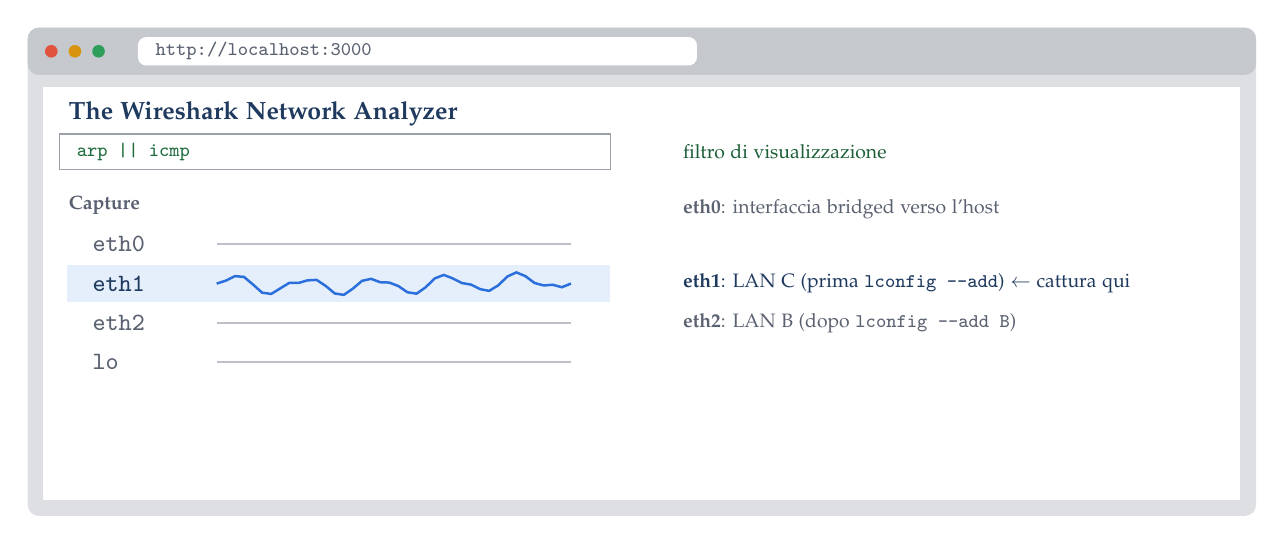
\begin{tikzpicture}[x=1cm,y=1cm]
  \fill[grigio!20,rounded corners=4pt] (0,0) rectangle (15.6,6.2);
  \fill[grigio!35,rounded corners=4pt] (0,5.6) rectangle (15.6,6.2);
  \foreach \c [count=\i] in {rosso,ambra,verde}{\fill[\c](\i*.3,5.9)circle(.08);}
  \fill[white,rounded corners=3pt] (1.4,5.72) rectangle (8.5,6.08);
  \node[anchor=west,font=\ttfamily\scriptsize,text=grigio] at (1.5,5.9) {http://localhost:3000};
  \fill[white] (.2,.2) rectangle (15.4,5.45);
  \node[anchor=west,font=\headfont\bfseries\small,text=navy] at (.4,5.1) {The Wireshark Network Analyzer};
  \draw[grigio!60] (.4,4.4) rectangle (7.4,4.85); \node[anchor=west,font=\ttfamily\scriptsize,text=verde!70!black] at (.5,4.62) {arp || icmp};
  \node[anchor=west,font=\headfont\scriptsize\bfseries,text=grigio] at (.4,3.95) {Capture};
  \foreach \y/\n/\c in {3.45/eth0/grigio,2.95/eth1/navy,2.45/eth2/grigio,1.95/lo/grigio}{
    \node[anchor=west,font=\ttfamily\small,text=\c] at (.7,\y) {\n};
    \draw[\c!40,line width=.8pt] (2.4,\y) -- (6.9,\y);
  }
  \fill[blu!12] (.5,2.72) rectangle (7.4,3.18);
  \node[anchor=west,font=\ttfamily\small\bfseries,text=navy] at (.7,2.95) {eth1};
  \draw[blu,line width=.9pt] plot[domain=0:4.5,samples=40] ({2.4+\x},{2.95+.15*sin(400*\x)*(abs(sin(170*\x)))});
  \node[anchor=west,font=\headfont\scriptsize,text=grigio,align=left] at (8.2,3.9) {\textbf{eth0}: interfaccia bridged verso l'host};
  \node[anchor=west,font=\headfont\scriptsize,text=navy,align=left] at (8.2,2.95) {\textbf{eth1}: LAN C (prima \texttt{lconfig --add}) $\leftarrow$ cattura qui};
  \node[anchor=west,font=\headfont\scriptsize,text=grigio,align=left] at (8.2,2.45) {\textbf{eth2}: LAN B (dopo \texttt{lconfig --add B})};
  \node[anchor=west,font=\headfont\scriptsize,text=verde!60!black,align=left] at (8.2,4.62) {filtro di visualizzazione};
\end{tikzpicture}
\end{center}
\didascalia{Schema dell'interfaccia web di Wireshark (illustrativo): si seleziona l'interfaccia del container collegata alla LAN da osservare. Il traffico di eth1 compare solo dopo aver collegato wireshark alla LAN C.}

\begin{attenzione}[Se la pagina non si apre]
Il container wireshark impiega qualche secondo a partire dopo \texttt{lstart}. Controlla che nessun altro programma usi la porta 3000 dell'host (è quella mappata da \texttt{wireshark[port]="3000:3000"}). Se \texttt{eth1} non compare nell'elenco, probabilmente non hai ancora eseguito \texttt{lconfig --add}.
\end{attenzione}

\begin{appunti}{Checklist di avvio}
\texttt{cd} nella cartella $\to$ \texttt{kathara lstart} $\to$ \texttt{ip a} su tutti (indirizzi giusti?) $\to$ \texttt{routel} sugli host (default gateway?) $\to$ \texttt{routel} sui router (2 reti dirette + 1 statica?) $\to$ \texttt{kathara lconfig -n wireshark --add C} $\to$ browser su \texttt{localhost:3000}, cattura su \texttt{eth1}.
\end{appunti}

\sezione{7}{Esperimento 1: ping nella stessa LAN e ARP}{da pc3 a pc2}

\subsection{Obiettivo e procedura}
Osservare cosa succede quando un host comunica con un vicino \textbf{della stessa LAN}: pc3 (\texttt{200.1.1.3}) fa ping a pc2 (\texttt{200.1.1.7}), entrambi sulla LAN C. Con wireshark collegato a C (capitolo 6, cattura su \texttt{eth1}), su \textbf{pc3}:
\begin{enumerate}
  \item ispeziona la cache ARP;
  \item esegui un ping verso pc2;
  \item ispeziona di nuovo la cache ARP;
  \item guarda i pacchetti catturati da Wireshark.
\end{enumerate}

\begin{center}
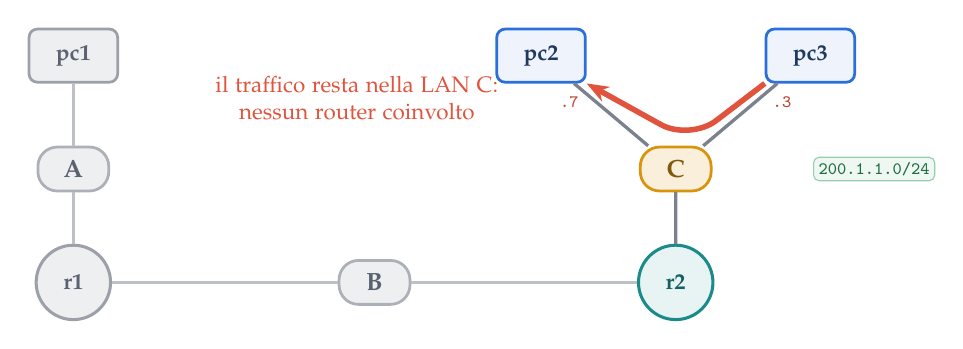
\begin{tikzpicture}[scale=.9,transform shape]
  \node[host,fill=grigio!10,draw=grigio!60,text=grigio] (pc1) at (0,3.2) {pc1};
  \node[rtr,fill=grigio!10,draw=grigio!60,text=grigio] (r1) at (0,0) {r1};
  \node[rtr] (r2) at (8.5,0) {r2};
  \node[host] (pc2) at (6.6,3.2) {pc2};
  \node[host] (pc3) at (10.4,3.2) {pc3};
  \node[cd,fill=grigio!10,draw=grigio!50,text=grigio] (A) at (0,1.6) {A};
  \node[cd,fill=grigio!10,draw=grigio!50,text=grigio] (B) at (4.25,0) {B};
  \node[cd] (C) at (8.5,1.6) {C};
  \draw[lnk,grigio!40] (pc1)--(A)--(r1)--(B)--(r2);
  \draw[lnk] (r2)--(C); \draw[lnk] (C)--(pc2); \draw[lnk] (C)--(pc3);
  \node[ipl] at (7.0,2.55) {.7}; \node[ipl] at (10.0,2.55) {.3};
  \draw[rosso,line width=2pt,-{Stealth[length=8pt]},rounded corners=12pt] (pc3.south west) -- (8.7,2.0) -- (pc2.south east);
  \node[netl] at (11.3,1.6) {200.1.1.0/24};
  \node[font=\headfont\small,text=rosso,align=center] at (4.0,2.6) {il traffico resta nella LAN C:\\nessun router coinvolto};
\end{tikzpicture}
\end{center}

\subsection{Cosa vedi nei terminali}
\begin{terminale}{pc3}
§root@pc3:/#§ arp -n                          °# 1) la cache ARP è inizialmente vuota°
§root@pc3:/#§ ping 200.1.1.7                  °# 2) invio richiede la risoluzione ARP°
PING 200.1.1.7 (200.1.1.7) 56(84) bytes of data.
64 bytes from 200.1.1.7: icmp_seq=1 ¤ttl=64¤ time=1.93 ms
64 bytes from 200.1.1.7: icmp_seq=2 ¤ttl=64¤ time=0.638 ms
^C
--- 200.1.1.7 ping statistics ---
2 packets transmitted, 2 received, 0% packet loss, time 1001ms
rtt min/avg/max/mdev = 0.638/1.283/1.929/0.645 ms
§root@pc3:/#§ arp -n                          °# 3) il risultato ARP è in cache°
Address        HWtype  HWaddress            Flags Mask  Iface
¤200.1.1.7      ether   00:00:00:00:00:02¤    C           eth0
\end{terminale}
\begin{esempio}[Cosa notare]
\begin{itemize}
  \item Prima del ping la cache è vuota: pc3 non ha mai parlato con nessuno.
  \item \texttt{ttl=64}: la risposta non ha attraversato alcun router.
  \item Il primo RTT (1.93\,ms) è più lungo del secondo (0.64\,ms): il primo pacchetto ha dovuto aspettare la risoluzione ARP.
  \item Dopo il ping la cache contiene il MAC di pc2 (\texttt{00:..:02}, quello forzato nel \texttt{lab.conf}).
\end{itemize}
\end{esempio}

\subsection{Cosa succede sulla rete: il diagramma temporale}
\begin{center}
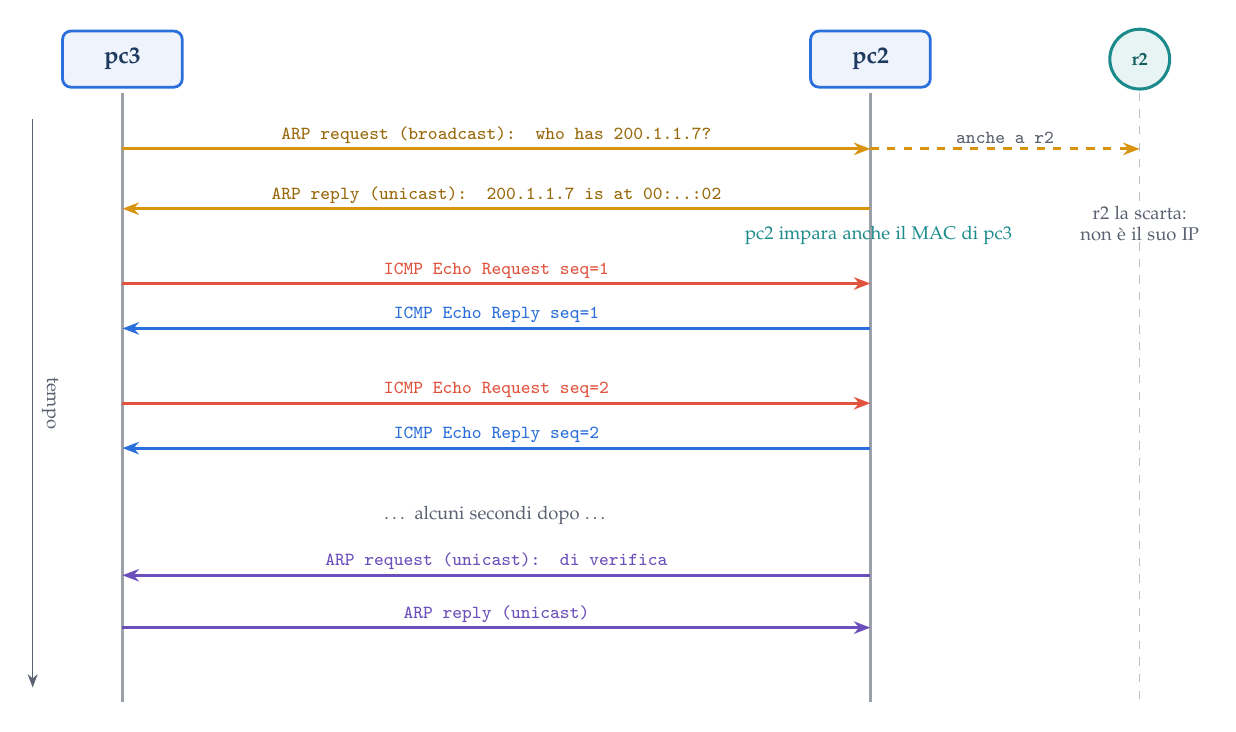
\begin{tikzpicture}[y=-1cm,scale=.95,transform shape,
  msg/.style={-{Stealth[length=6pt]},line width=1.1pt},
  ml/.style={font=\ttfamily\scriptsize,fill=white,inner sep=1.5pt}]
  \foreach \x/\n in {0/pc3,10/pc2}{
    \node[host,minimum width=1.6cm] at (\x,0) {\n};
    \draw[grigio!60,line width=1pt] (\x,.45) -- (\x,8.6);
  }
  \node[rtr,minimum size=.8cm,font=\headfont\bfseries\scriptsize] at (13.6,0) {r2};
  \draw[grigio!40,dashed] (13.6,.45) -- (13.6,8.6);
  \draw[-{Stealth},grigio] (-1.2,.8) -- node[sloped,above,font=\headfont\scriptsize]{tempo} (-1.2,8.4);
  % arp broadcast
  \draw[msg,ambra] (0,1.2) -- node[ml,above,text=ambra!70!black]{ARP request (broadcast): who has 200.1.1.7?} (10,1.2);
  \draw[msg,ambra,dashed] (10,1.2) -- node[ml,above,text=grigio]{anche a r2} (13.6,1.2);
  \node[font=\headfont\scriptsize,text=grigio,align=center] at (13.6,2.2) {r2 la scarta:\\non è il suo IP};
  \draw[msg,ambra] (10,2.0) -- node[ml,above,text=ambra!70!black]{ARP reply (unicast): 200.1.1.7 is at 00:..:02} (0,2.0);
  \node[font=\headfont\scriptsize,text=teal,anchor=west] at (8.2,2.35) {pc2 impara anche il MAC di pc3};
  \draw[msg,rosso] (0,3.0) -- node[ml,above,text=rosso]{ICMP Echo Request seq=1} (10,3.0);
  \draw[msg,blu] (10,3.6) -- node[ml,above,text=blu]{ICMP Echo Reply seq=1} (0,3.6);
  \draw[msg,rosso] (0,4.6) -- node[ml,above,text=rosso]{ICMP Echo Request seq=2} (10,4.6);
  \draw[msg,blu] (10,5.2) -- node[ml,above,text=blu]{ICMP Echo Reply seq=2} (0,5.2);
  \node[font=\headfont\scriptsize,text=grigio] at (5,6.1) {\dots{} alcuni secondi dopo \dots};
  \draw[msg,viola] (10,6.9) -- node[ml,above,text=viola]{ARP request (unicast): di verifica} (0,6.9);
  \draw[msg,viola] (0,7.6) -- node[ml,above,text=viola]{ARP reply (unicast)} (10,7.6);
\end{tikzpicture}
\end{center}

\subsection{La cattura in Wireshark}
\begin{center}
\footnotesize\ttfamily
\setlength{\tabcolsep}{4pt}
\begin{tabularx}{\linewidth}{r l l l l >{\raggedright\arraybackslash}X}
\rowcolor{navy}\thd{No.} & \thd{Source} & \thd{Destination} & \thd{Proto} & \thd{TTL} & \thd{Info}\\
\wsrow{1}{00:..:00:03}{Broadcast}{ARP}{}{Who has 200.1.1.7? Tell 200.1.1.3}{ambra!18}
\wsrow{2}{00:..:00:02}{00:..:00:03}{ARP}{}{200.1.1.7 is at 00:00:00:00:00:02}{ambra!18}
\wsrow{3}{200.1.1.3}{200.1.1.7}{ICMP}{64}{Echo (ping) request seq=1}{rosso!10}
\wsrow{4}{200.1.1.7}{200.1.1.3}{ICMP}{64}{Echo (ping) reply seq=1}{rosso!10}
\wsrow{5}{200.1.1.3}{200.1.1.7}{ICMP}{64}{Echo (ping) request seq=2}{rosso!10}
\wsrow{6}{200.1.1.7}{200.1.1.3}{ICMP}{64}{Echo (ping) reply seq=2}{rosso!10}
\wsrow{7}{00:..:00:02}{00:..:00:03}{ARP}{}{Who has 200.1.1.3? Tell 200.1.1.7}{viola!10}
\wsrow{8}{00:..:00:03}{00:..:00:02}{ARP}{}{200.1.1.3 is at 00:00:00:00:00:03}{viola!10}
\end{tabularx}
\end{center}
\didascalia{Ricostruzione illustrativa della lista pacchetti sulla LAN C (i colori imitano quelli di Wireshark: giallo per ARP, rosa per ICMP). Gli ultimi due frame sono il dialogo ARP unicast che avviene al termine del ping; quale dei due host lo avvia può variare.}

\begin{tecnica}[Dentro i frame ARP]
\begin{center}
\rowcolors{2}{chiaro}{white}
\begin{tabular}{l l l}
\rowcolor{navy}\thd{Campo} & \thd{ARP request (frame 1)} & \thd{ARP reply (frame 2)}\\
Ethernet destinazione & \texttt{ff:ff:ff:ff:ff:ff} (broadcast) & \texttt{00:00:00:00:00:03} (pc3)\\
Ethernet sorgente & \texttt{00:00:00:00:00:03} & \texttt{00:00:00:00:00:02}\\
Opcode & 1 (request) & 2 (reply)\\
Sender MAC / IP & \texttt{00:..:03} / \texttt{200.1.1.3} & \texttt{00:..:02} / \texttt{200.1.1.7}\\
Target MAC / IP & \texttt{00:00:00:00:00:00} (ignoto) / \texttt{200.1.1.7} & \texttt{00:..:03} / \texttt{200.1.1.3}\\
\end{tabular}
\end{center}
La request va in \textbf{broadcast} perché pc3 non sa ancora a chi mandarla: la ricevono tutti i dispositivi della LAN C (pc2, r2 e wireshark), ma risponde solo chi possiede l'IP cercato. La reply è \textbf{unicast}: pc2 sa già chi ha chiesto, perché il MAC di pc3 è scritto nella request.
\end{tecnica}

\subsection{pc2 impara senza chiedere}
\begin{terminale}{pc2}
§root@pc2:/#§ arp -n
Address        HWtype  HWaddress            Flags Mask  Iface
¤200.1.1.3      ether   00:00:00:00:00:03¤    C           eth0
\end{terminale}
\begin{intuizione}
pc2 non ha mai inviato una ARP request, eppure conosce il MAC di pc3. Le comunicazioni sono quasi sempre \textbf{bidirezionali}: chi riceve una ARP request rivolta a sé memorizza subito il MAC di chi l'ha mandata, perché quasi certamente dovrà rispondergli (qui con gli Echo Reply). Così si evita una seconda risoluzione ARP nel verso opposto. È il comportamento standard previsto dall'RFC 826.
\end{intuizione}
\begin{mlbox}[Il dialogo ARP unicast finale]
Le voci della cache ARP non sono eterne. In Linux, dopo un po' di tempo senza conferme, una voce passa dallo stato \texttt{REACHABLE} a \texttt{STALE}; quando la si riusa, il kernel la \emph{verifica} con una ARP request \textbf{unicast} direttamente al MAC già noto, invece di un nuovo broadcast. È il meccanismo di \emph{neighbour unreachability detection}. Puoi seguire gli stati con \inl{ip neigh} mentre il ping è in corso e subito dopo.
\end{mlbox}

\begin{appunti}{Riepilogo dell'esperimento 1}
Stessa LAN $\Rightarrow$ nessun router, \texttt{ttl=64}. Prima del primo pacchetto IP: ARP request \textbf{broadcast} (ricevuta da tutti su C) e ARP reply \textbf{unicast}. Il risultato va in cache (\texttt{arp -n}). Chi riceve la request impara il MAC del richiedente (RFC 826): pc2 ha pc3 in cache senza aver chiesto. Alla fine: ARP unicast di verifica della voce in cache.
\end{appunti}

\sezione{8}{Esperimento 2: ping attraverso i router}{da pc2 a pc1}

\subsection{Obiettivo e procedura}
Ora la destinazione è \textbf{fuori dalla LAN} del mittente: pc2 (\texttt{200.1.1.7}, LAN C) fa ping a pc1 (\texttt{195.11.14.5}, LAN A). Il pacchetto deve attraversare r2 e r1. Per osservare il tratto centrale si collega wireshark anche alla LAN B:
\begin{terminale}{host}
§user@localhost:~/kathara-lab_basic-ipv4$§ kathara lconfig -n wireshark --add B
\end{terminale}
Nel browser (\texttt{localhost:3000}) si cattura su \textbf{\texttt{eth2}}, la seconda interfaccia aggiunta. Poi, su pc2:
\begin{terminale}{pc2}
§root@pc2:/#§ ping 195.11.14.5
PING 195.11.14.5 (195.11.14.5) 56(84) bytes of data.
64 bytes from 195.11.14.5: icmp_seq=1 ¤ttl=62¤ time=5.86 ms
64 bytes from 195.11.14.5: icmp_seq=2 ¤ttl=62¤ time=1.69 ms
^C
--- 195.11.14.5 ping statistics ---
2 packets transmitted, 2 received, 0% packet loss, time 1002ms
rtt min/avg/max/mdev = 1.688/3.771/5.855/2.083 ms
\end{terminale}
\texttt{ttl=62}: la risposta di pc1 è partita con TTL 64 ed è stata decrementata da r1 e da r2. Il primo RTT (5.86\,ms) è più alto perché sul percorso servono ben tre risoluzioni ARP.

\begin{center}
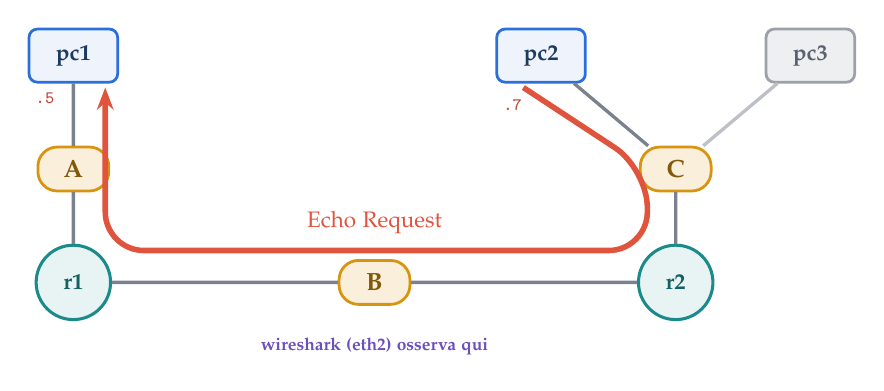
\begin{tikzpicture}[scale=.9,transform shape]
  \node[host] (pc1) at (0,3.2) {pc1};
  \node[rtr] (r1) at (0,0) {r1};
  \node[rtr] (r2) at (8.5,0) {r2};
  \node[host] (pc2) at (6.6,3.2) {pc2};
  \node[host,fill=grigio!10,draw=grigio!60,text=grigio] (pc3) at (10.4,3.2) {pc3};
  \node[cd] (A) at (0,1.6) {A};
  \node[cd] (B) at (4.25,0) {B};
  \node[cd] (C) at (8.5,1.6) {C};
  \draw[lnk] (pc1)--(A)--(r1)--(B)--(r2)--(C)--(pc2); \draw[lnk,grigio!40] (C)--(pc3);
  \draw[rosso,line width=2pt,-{Stealth[length=8pt]},rounded corners=14pt] (6.35,2.75) -- (8.1,1.6) -- (8.1,.45) -- (.45,.45) -- (.45,2.75);
  \node[font=\headfont\small,text=rosso] at (4.25,.85) {Echo Request};
  \node[viola,font=\headfont\scriptsize\bfseries] at (4.25,-.9) {wireshark (eth2) osserva qui};
  \node[ipl] at (6.2,2.5) {.7}; \node[ipl] at (-.4,2.6) {.5};
\end{tikzpicture}
\end{center}

\subsection{La regola fondamentale: l'host decide se consegnare o delegare}
\begin{intuizione}
Prima di spedire, pc2 confronta la destinazione con la propria rete: \texttt{195.11.14.5} \emph{non} appartiene a \texttt{200.1.1.0/24}. Allora non cerca il MAC di pc1 (che non riceverebbe mai la sua ARP request: i broadcast \textbf{non attraversano i router}). Cerca invece il MAC del suo \textbf{default gateway}, \texttt{200.1.1.1} (r2), e gli consegna il pacchetto. Ogni router ripete lo stesso ragionamento con la propria tabella di routing.
\end{intuizione}
\begin{center}
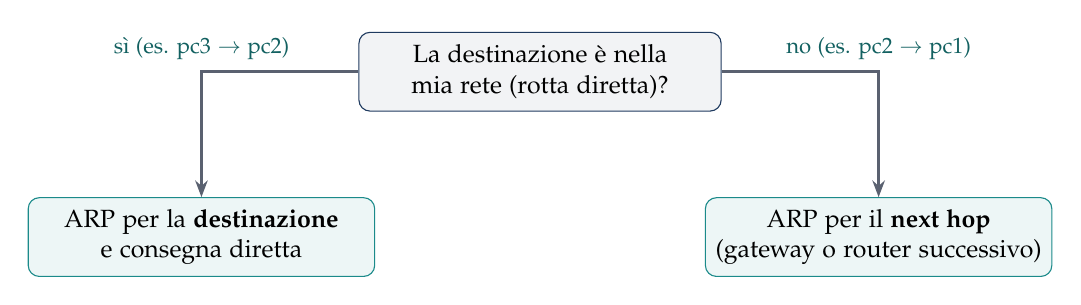
\begin{tikzpicture}[
  q/.style={draw=navy,fill=navy!6,rounded corners=4pt,align=center,font=\headfont\small,minimum width=4.6cm,minimum height=1cm},
  a/.style={draw=teal,fill=teal!8,rounded corners=4pt,align=center,font=\headfont\small,minimum width=4.4cm,minimum height=1cm},
  ar/.style={-{Stealth[length=6pt]},line width=1pt,color=grigio}]
  \node[q] (d) at (0,0) {La destinazione è nella\\mia rete (rotta diretta)?};
  \node[a] (y) at (-4.3,-2.1) {ARP per la \textbf{destinazione}\\e consegna diretta};
  \node[a] (n) at (4.3,-2.1) {ARP per il \textbf{next hop}\\(gateway o router successivo)};
  \draw[ar] (d.west) -| (y.north);
  \draw[ar] (d.east) -| (n.north);
  \node[font=\headfont\footnotesize,text=teal!70!black] at (-4.3,.3) {sì (es. pc3 $\to$ pc2)};
  \node[font=\headfont\footnotesize,text=teal!70!black] at (4.3,.3) {no (es. pc2 $\to$ pc1)};
\end{tikzpicture}
\end{center}

\subsection{Le cache ARP dopo il ping}
\begin{terminale}{pc2}
§root@pc2:/#§ arp -n
Address        HWtype  HWaddress            Flags Mask  Iface
¤200.1.1.1      ether   00:00:00:00:00:c1¤    C           eth0     °# r2, il gateway°
200.1.1.3      ether   00:00:00:00:00:03    C           eth0     °# pc3, dall'esperimento 1°
\end{terminale}
pc2 conosce il MAC di \texttt{eth0} di \textbf{r2}, non quello di pc1. Anche i router fanno ARP, ogni volta che devono spedire pacchetti IP su una LAN Ethernet:
\begin{terminale}{r1}
§root@r1:/#§ arp -n
Address        HWtype  HWaddress            Flags Mask  Iface
195.11.14.5    ether   00:00:00:00:00:01    C           eth0     °# pc1°
100.0.0.10     ether   00:00:00:00:00:b2    C           eth1     °# r2 (eth1)°
\end{terminale}
\begin{terminale}{r2}
§root@r2:/#§ arp -n
Address        HWtype  HWaddress            Flags Mask  Iface
100.0.0.9      ether   00:00:00:00:00:b1    C           eth1     °# r1 (eth1)°
200.1.1.7      ether   00:00:00:00:00:02    C           eth0     °# pc2°
\end{terminale}
\begin{tecnica}[Ogni cache contiene solo vicini della stessa LAN]
Nessuno conosce il MAC di un dispositivo che sta su un'altra LAN: pc2 non ha mai visto \texttt{00:..:01}, pc1 non ha mai visto \texttt{00:..:02}. Ogni voce ARP è legata all'interfaccia (\texttt{Iface}) su cui il vicino è raggiungibile.
\end{tecnica}

\subsection{Cosa cambia a ogni salto}
\begin{center}
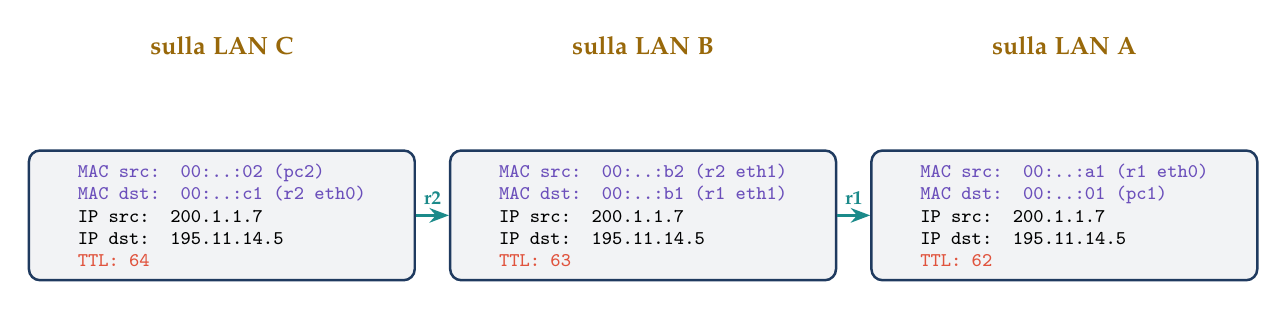
\begin{tikzpicture}[
  pk/.style={rounded corners=4pt,draw=#1,fill=#1!6,line width=.9pt,minimum width=4.9cm,align=left,font=\ttfamily\scriptsize,inner sep=5pt},
  hd/.style={font=\headfont\bfseries\small}]
  \node[hd,text=ambra!70!black] at (0,2.15) {sulla LAN C};
  \node[hd,text=ambra!70!black] at (5.35,2.15) {sulla LAN B};
  \node[hd,text=ambra!70!black] at (10.7,2.15) {sulla LAN A};
  \node[pk=navy] (c) at (0,0) {\textcolor{viola}{MAC src: 00:..:02 (pc2)}\\\textcolor{viola}{MAC dst: 00:..:c1 (r2 eth0)}\\IP  src: 200.1.1.7\\IP  dst: 195.11.14.5\\\textcolor{rosso}{TTL: 64}};
  \node[pk=navy] (b) at (5.35,0) {\textcolor{viola}{MAC src: 00:..:b2 (r2 eth1)}\\\textcolor{viola}{MAC dst: 00:..:b1 (r1 eth1)}\\IP  src: 200.1.1.7\\IP  dst: 195.11.14.5\\\textcolor{rosso}{TTL: 63}};
  \node[pk=navy] (a) at (10.7,0) {\textcolor{viola}{MAC src: 00:..:a1 (r1 eth0)}\\\textcolor{viola}{MAC dst: 00:..:01 (pc1)}\\IP  src: 200.1.1.7\\IP  dst: 195.11.14.5\\\textcolor{rosso}{TTL: 62}};
  \draw[-{Stealth[length=7pt]},line width=1.3pt,teal] (c.east) -- node[above,font=\headfont\bfseries\scriptsize]{r2} (b.west);
  \draw[-{Stealth[length=7pt]},line width=1.3pt,teal] (b.east) -- node[above,font=\headfont\bfseries\scriptsize]{r1} (a.west);
\end{tikzpicture}
\end{center}
\didascalia{L'Echo Request nelle tre LAN: gli indirizzi \textbf{IP} restano gli stessi dall'inizio alla fine, i \textbf{MAC} cambiano a ogni LAN (riscritti da ciascun router) e il \textbf{TTL} scende di 1 a ogni router.}

\subsection{La cattura sulla LAN B}
\begin{center}
\footnotesize\ttfamily
\setlength{\tabcolsep}{4pt}
\begin{tabularx}{\linewidth}{r l l l l >{\raggedright\arraybackslash}X}
\rowcolor{navy}\thd{No.} & \thd{Source} & \thd{Destination} & \thd{Proto} & \thd{TTL} & \thd{Info}\\
\wsrow{1}{00:..:00:b2}{Broadcast}{ARP}{}{Who has 100.0.0.9? Tell 100.0.0.10}{ambra!18}
\wsrow{2}{00:..:00:b1}{00:..:00:b2}{ARP}{}{100.0.0.9 is at 00:..:00:b1 \textrm{(r1)}}{ambra!18}
\wsrow{3}{200.1.1.7}{195.11.14.5}{ICMP}{63}{Echo (ping) request seq=1}{rosso!10}
\wsrow{4}{195.11.14.5}{200.1.1.7}{ICMP}{63}{Echo (ping) reply seq=1}{rosso!10}
\wsrow{5}{200.1.1.7}{195.11.14.5}{ICMP}{63}{Echo (ping) request seq=2}{rosso!10}
\wsrow{6}{195.11.14.5}{200.1.1.7}{ICMP}{63}{Echo (ping) reply seq=2}{rosso!10}
\end{tabularx}
\end{center}
\didascalia{Ricostruzione illustrativa. Sulla LAN B gli indirizzi IP sono quelli di pc2 e pc1, ma nessuno dei due è collegato a B: i frame passano tra i MAC \texttt{b1} e \texttt{b2} dei router. Il TTL vale 63 in entrambe le direzioni perché ogni pacchetto ha già attraversato un router.}

\subsection{Il quadro completo}
\begin{center}
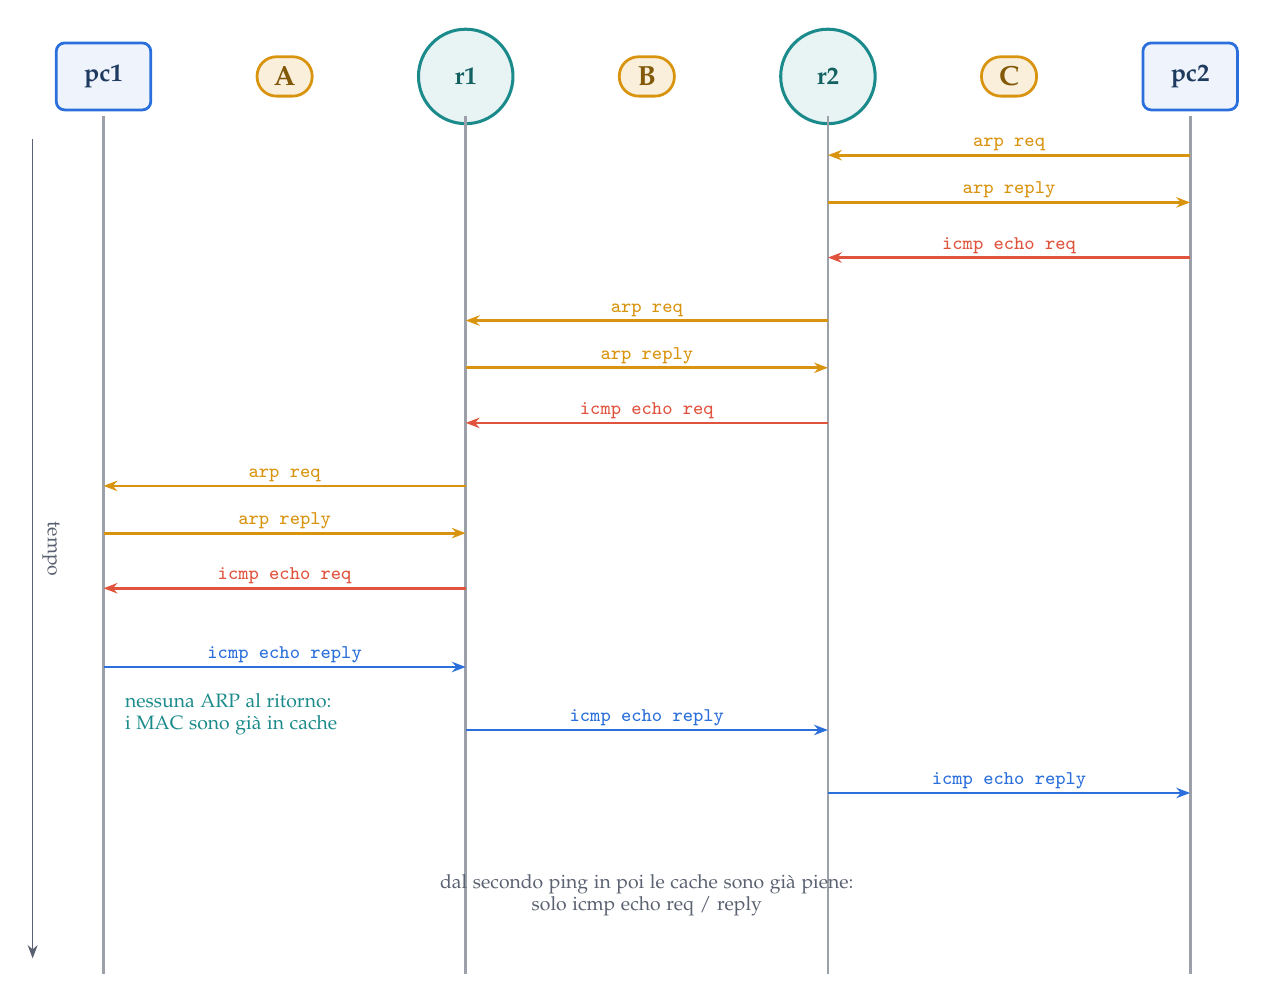
\begin{tikzpicture}[y=-1cm,x=1cm,
  msg/.style={-{Stealth[length=5pt]},line width=1pt},
  ml/.style={font=\ttfamily\scriptsize,fill=white,inner sep=1pt}]
  \foreach \x/\n/\s in {0/pc1/host,4.6/r1/rtr,9.2/r2/rtr,13.8/pc2/host}{
    \node[\s,minimum size=.85cm,minimum width=1.2cm] at (\x,0) {\n};
    \draw[grigio!60,line width=1pt] (\x,.5) -- (\x,11.4);
  }
  \foreach \x/\l in {2.3/A,6.9/B,11.5/C}{\node[cd,minimum width=.7cm,minimum height=.5cm] at (\x,0) {\l};}
  \draw[-{Stealth},grigio] (-.9,.8) -- node[sloped,above,font=\headfont\scriptsize]{tempo} (-.9,11.2);
  % pc2 -> r2
  \draw[msg,ambra] (13.8,1.0) -- node[ml,above]{arp req} (9.2,1.0);
  \draw[msg,ambra] (9.2,1.6) -- node[ml,above]{arp reply} (13.8,1.6);
  \draw[msg,rosso] (13.8,2.3) -- node[ml,above]{icmp echo req} (9.2,2.3);
  % r2 -> r1
  \draw[msg,ambra] (9.2,3.1) -- node[ml,above]{arp req} (4.6,3.1);
  \draw[msg,ambra] (4.6,3.7) -- node[ml,above]{arp reply} (9.2,3.7);
  \draw[msg,rosso] (9.2,4.4) -- node[ml,above]{icmp echo req} (4.6,4.4);
  % r1 -> pc1
  \draw[msg,ambra] (4.6,5.2) -- node[ml,above]{arp req} (0,5.2);
  \draw[msg,ambra] (0,5.8) -- node[ml,above]{arp reply} (4.6,5.8);
  \draw[msg,rosso] (4.6,6.5) -- node[ml,above]{icmp echo req} (0,6.5);
  % replies
  \draw[msg,blu] (0,7.5) -- node[ml,above]{icmp echo reply} (4.6,7.5);
  \draw[msg,blu] (4.6,8.3) -- node[ml,above]{icmp echo reply} (9.2,8.3);
  \draw[msg,blu] (9.2,9.1) -- node[ml,above]{icmp echo reply} (13.8,9.1);
  \node[font=\headfont\scriptsize,text=teal,align=left,anchor=west] at (.15,8.1) {nessuna ARP al ritorno:\\i MAC sono già in cache};
  \node[font=\headfont\scriptsize,text=grigio,align=center] at (6.9,10.4) {dal secondo ping in poi le cache sono già piene:\\solo icmp echo req / reply};
\end{tikzpicture}
\end{center}
\didascalia{Primo ping da pc2 a pc1: ogni tratto richiede prima una risoluzione ARP. Le risposte non generano nuove ARP, perché chi ha ricevuto una ARP request ha già memorizzato il MAC del richiedente.}

\begin{appunti}{Riepilogo dell'esperimento 2}
Destinazione fuori LAN $\Rightarrow$ l'host fa ARP per il \textbf{default gateway}, non per la destinazione (ARP non attraversa i router). Ogni router fa ARP per il next hop. IP src/dst invariati, MAC riscritti a ogni LAN, TTL $-1$ per router (\texttt{ttl=62} = 2 router). Cache: pc2 $\to$ r2 (\texttt{c1}); r2 $\to$ r1 (\texttt{b1}), pc2; r1 $\to$ r2 (\texttt{b2}), pc1. wireshark su B: \texttt{lconfig --add B}, cattura su \texttt{eth2}.
\end{appunti}

\sezione{9}{Esperimento 3: traceroute}{da pc2 a pc1}

\subsection{Obiettivo e procedura}
Scoprire \textbf{quali router} attraversa un pacchetto da pc2 a pc1 e capire \emph{come} traceroute ricava questa informazione. wireshark è già collegato alla LAN C: nel browser si cattura su \texttt{eth1}. Su pc2:
\begin{terminale}{pc2}
§root@pc2:/#§ traceroute 195.11.14.5 -z 1
traceroute to 195.11.14.5 (195.11.14.5), 30 hops max, 60 byte packets
 1  ¤200.1.1.1¤ (200.1.1.1)  0.882 ms  0.662 ms  0.456 ms      °# eth0 di r2°
 2  ¤100.0.0.9¤ (100.0.0.9)  0.903 ms  0.877 ms  1.218 ms      °# eth1 di r1°
 3  ¤195.11.14.5¤ (195.11.14.5)  0.987 ms  1.354 ms  1.015 ms  °# eth0 di pc1°
\end{terminale}
\begin{esempio}[Come si legge]
\begin{itemize}
  \item \texttt{30 hops max}: prova al massimo fino a TTL 30. \texttt{60 byte packets}: dimensione delle sonde.
  \item Ogni riga è un \textbf{salto}: il numero è il TTL usato, poi l'indirizzo che ha risposto e tre tempi (una per ciascuna delle 3 sonde).
  \item L'indirizzo mostrato per un router è quello dell'interfaccia \textbf{da cui ha inviato la risposta} verso pc2: per r2 è \texttt{200.1.1.1} (eth0, lato C), per r1 è \texttt{100.0.0.9} (eth1, lato B). Non sono le interfacce «verso pc1»!
  \item \texttt{-z 1}: attende 1 secondo tra una sonda e l'altra, così in Wireshark i pacchetti sono ben separati.
\end{itemize}
\end{esempio}

\subsection{Il trucco del TTL}
\begin{intuizione}
Ogni pacchetto IP ha un \textbf{TTL} (\emph{Time To Live}), un contatore che ogni router decrementa di 1. Se arriva a 0, il router butta il pacchetto e avvisa il mittente con un messaggio ICMP \textbf{Time Exceeded} (\emph{time-to-live exceeded in transit}), che porta il proprio indirizzo come sorgente. Serve a impedire che i pacchetti girino all'infinito in caso di cicli di routing.

traceroute sfrutta questo meccanismo «di proposito»: manda sonde con TTL = 1, poi 2, poi 3\dots{} La sonda con TTL = $k$ «muore» esattamente al $k$-esimo router, che si rivela rispondendo.
\end{intuizione}
\begin{center}
\rowcolors{2}{chiaro}{white}
\begin{tabularx}{\linewidth}{c l Y l}
\rowcolor{navy}\thd{TTL sonda} & \thd{Dove si ferma} & \thd{Cosa succede} & \thd{Risposta}\\
1 & r2 & r2 decrementa a 0, scarta la sonda & ICMP Time Exceeded da 200.1.1.1\\
2 & r1 & r2 porta il TTL a 1, r1 a 0 e scarta & ICMP Time Exceeded da 100.0.0.9\\
3 & pc1 & arriva a pc1 con TTL 1: è la destinazione & ICMP Port Unreachable da 195.11.14.5\\
\end{tabularx}
\end{center}
\begin{tecnica}[Perché la destinazione risponde «Port Unreachable»]
Le sonde di traceroute (versione Linux, default) sono datagrammi \textbf{UDP} indirizzati a pc1 su porte alte (a partire da 33434) dove con ogni probabilità nessun programma è in ascolto. Quando una sonda arriva davvero a pc1, il kernel di pc1 risponde con ICMP \textbf{Destination Unreachable / Port Unreachable}. Per traceroute questo è il segnale che la destinazione è stata raggiunta e che può fermarsi.
\end{tecnica}

\subsection{La cattura sulla LAN C}
\begin{center}
\footnotesize\ttfamily
\setlength{\tabcolsep}{4pt}
\begin{tabularx}{\linewidth}{r l l l l >{\raggedright\arraybackslash}X}
\rowcolor{navy}\thd{No.} & \thd{Source} & \thd{Destination} & \thd{Proto} & \thd{TTL} & \thd{Info}\\
\wsrow{1}{200.1.1.7}{195.11.14.5}{UDP}{1}{33434 $\rightarrow$ ... sonda 1/3}{blu!8}
\wsrow{2}{200.1.1.1}{200.1.1.7}{ICMP}{64}{Time-to-live exceeded (in transit)}{rosso!20}
\wsrow{\dots}{}{}{}{}{\textrm{altre 2 sonde con TTL=1 e relative risposte}}{white}
\wsrow{7}{200.1.1.7}{195.11.14.5}{UDP}{2}{sonda con TTL=2}{blu!8}
\wsrow{8}{100.0.0.9}{200.1.1.7}{ICMP}{63}{Time-to-live exceeded (in transit)}{rosso!20}
\wsrow{\dots}{}{}{}{}{\textrm{altre 2 sonde con TTL=2}}{white}
\wsrow{13}{200.1.1.7}{195.11.14.5}{UDP}{3}{sonda con TTL=3}{blu!8}
\wsrow{14}{195.11.14.5}{200.1.1.7}{ICMP}{62}{Destination unreachable (Port unreachable) \textrm{$\leftarrow$ destinazione raggiunta!}}{rosso!12}
\end{tabularx}
\end{center}
\didascalia{Ricostruzione illustrativa (numerazione indicativa). In Wireshark i messaggi ICMP di errore sono evidenziati con righe scure. Il campo \emph{Time to live} della sonda si legge nel dettaglio del pacchetto (header IP): 1, poi 2, poi 3. Durante il dialogo compaiono anche ARP unicast di verifica delle cache.}
\begin{attenzione}[Le righe scure in Wireshark non sono errori di cattura]
Wireshark colora in nero/rosso i pacchetti ICMP di errore (Time Exceeded, Destination Unreachable). Qui sono \emph{attesi}: sono proprio le risposte su cui si basa traceroute.
\end{attenzione}

\subsection{Il quadro completo}
\begin{center}
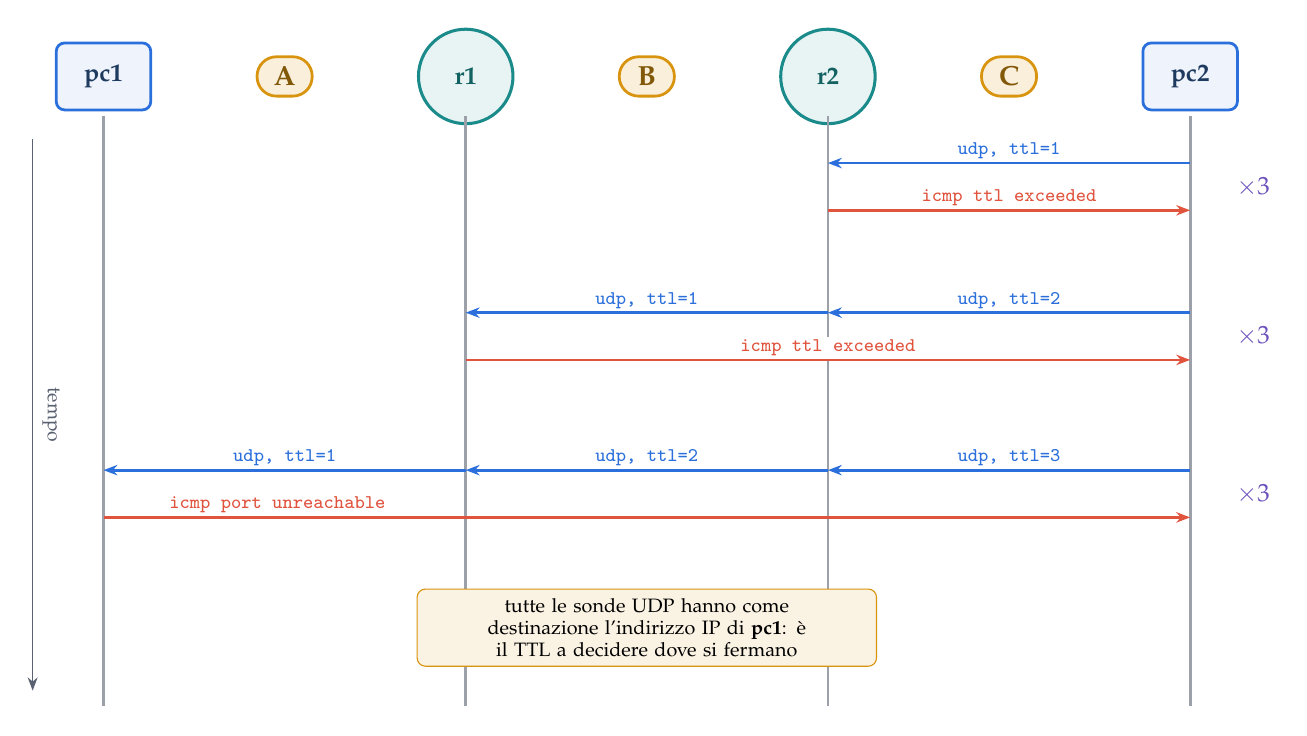
\begin{tikzpicture}[y=-1cm,x=1cm,
  msg/.style={-{Stealth[length=5pt]},line width=1pt},
  ml/.style={font=\ttfamily\scriptsize,fill=white,inner sep=1pt}]
  \foreach \x/\n/\s in {0/pc1/host,4.6/r1/rtr,9.2/r2/rtr,13.8/pc2/host}{
    \node[\s,minimum size=.85cm,minimum width=1.2cm] at (\x,0) {\n};
    \draw[grigio!60,line width=1pt] (\x,.5) -- (\x,8.0);
  }
  \foreach \x/\l in {2.3/A,6.9/B,11.5/C}{\node[cd,minimum width=.7cm,minimum height=.5cm] at (\x,0) {\l};}
  \draw[-{Stealth},grigio] (-.9,.8) -- node[sloped,above,font=\headfont\scriptsize]{tempo} (-.9,7.8);
  % ttl 1
  \draw[msg,blu] (13.8,1.1) -- node[ml,above]{udp, ttl=1} (9.2,1.1);
  \draw[msg,rosso] (9.2,1.7) -- node[ml,above]{icmp ttl exceeded} (13.8,1.7);
  \node[font=\headfont\bfseries\small,text=viola] at (14.6,1.4) {$\times3$};
  % ttl 2
  \draw[msg,blu] (13.8,3.0) -- node[ml,above]{udp, ttl=2} (9.2,3.0);
  \draw[msg,blu] (9.2,3.0) -- node[ml,above]{udp, ttl=1} (4.6,3.0);
  \draw[msg,rosso] (4.6,3.6) -- node[ml,above]{icmp ttl exceeded} (13.8,3.6);
  \node[font=\headfont\bfseries\small,text=viola] at (14.6,3.3) {$\times3$};
  % ttl 3
  \draw[msg,blu] (13.8,5.0) -- node[ml,above]{udp, ttl=3} (9.2,5.0);
  \draw[msg,blu] (9.2,5.0) -- node[ml,above]{udp, ttl=2} (4.6,5.0);
  \draw[msg,blu] (4.6,5.0) -- node[ml,above]{udp, ttl=1} (0,5.0);
  \draw[msg,rosso] (0,5.6) -- node[ml,above,pos=.16]{icmp port unreachable} (13.8,5.6);
  \node[font=\headfont\bfseries\small,text=viola] at (14.6,5.3) {$\times3$};
  \node[draw=ambra,fill=ambra!12,rounded corners=3pt,font=\headfont\scriptsize,align=center,text width=5.6cm] at (6.9,7.0) {tutte le sonde UDP hanno come destinazione l'indirizzo IP di \textbf{pc1}: è il TTL a decidere dove si fermano};
\end{tikzpicture}
\end{center}
\didascalia{Per ogni valore di TTL partono 3 sonde ($\times3$). Il TTL indicato sulle frecce è quello del pacchetto in ciascun tratto, dopo i decrementi dei router.}

\begin{mlbox}[Varianti utili]
\begin{itemize}
  \item \inl{traceroute -n 195.11.14.5}: niente risoluzione dei nomi (output più rapido).
  \item \inl{traceroute -I 195.11.14.5}: sonde ICMP Echo invece di UDP; la destinazione risponde con Echo Reply.
  \item Un asterisco \texttt{*} al posto del tempo significa «nessuna risposta entro il timeout»: router che non invia ICMP, filtro, o rotta di ritorno mancante.
\end{itemize}
\end{mlbox}

\begin{appunti}{Riepilogo dell'esperimento 3}
traceroute = sonde UDP verso la destinazione con TTL 1, 2, 3\dots{} (3 sonde per TTL). Ogni router che porta il TTL a 0 risponde \textbf{ICMP Time Exceeded} (rivela il suo indirizzo, quello dell'interfaccia da cui risponde). La destinazione risponde \textbf{ICMP Port Unreachable} (porta UDP chiusa): fine. Output pc2$\to$pc1: 200.1.1.1 (r2), 100.0.0.9 (r1), 195.11.14.5 (pc1). \texttt{-z 1}: 1\,s tra le sonde.
\end{appunti}

\sezione{10}{Esercizi guidati}{con soluzioni}

Gli esercizi 1 e 2 sono quelli proposti alla fine del lab; gli altri servono a fissare i comandi. Prova prima da solo, poi confronta con la soluzione. Se rompi qualcosa, \texttt{kathara lrestart} riporta tutto allo stato iniziale.

\subsection{Esercizio 1: destinazione irraggiungibile nella stessa LAN}
\begin{esempio}[Consegna]
Da pc3 fai ping a un indirizzo della LAN C che \textbf{non esiste}, per esempio \texttt{200.1.1.99}. Che messaggio ottieni? Quali pacchetti vedi sulla LAN C (wireshark su \texttt{eth1})?
\end{esempio}
\begin{terminale}{pc3}
§root@pc3:/#§ ping -c 4 200.1.1.99
PING 200.1.1.99 (200.1.1.99) 56(84) bytes of data.
From ¤200.1.1.3¤ icmp_seq=1 ¤Destination Host Unreachable¤
From 200.1.1.3 icmp_seq=2 Destination Host Unreachable
From 200.1.1.3 icmp_seq=3 Destination Host Unreachable
--- 200.1.1.99 ping statistics ---
4 packets transmitted, 0 received, +3 errors, 100% packet loss, time 3060ms
\end{terminale}
\begin{tecnica}[Soluzione]
\begin{itemize}
  \item La destinazione è nella LAN di pc3, quindi pc3 prova a risolverla con ARP: sulla LAN C compaiono solo \textbf{ARP request broadcast} ripetute («Who has 200.1.1.99? Tell 200.1.1.3»), senza alcuna reply.
  \item Senza MAC di destinazione pc3 non può costruire il frame Ethernet: \textbf{nessun pacchetto ICMP Echo esce sulla rete}.
  \item L'errore \texttt{Destination Host Unreachable} è generato \textbf{localmente} da pc3 stesso, infatti il mittente indicato è \texttt{200.1.1.3}, e arriva dopo qualche secondo (il tempo dei tentativi ARP).
\end{itemize}
\end{tecnica}

\subsection{Esercizio 2: destinazione irraggiungibile in un'altra LAN}
\begin{esempio}[Consegna]
Da pc2 fai ping a un host inesistente della LAN A (\texttt{195.11.14.99}) e poi a una rete che nessuno conosce (\texttt{8.8.8.8}). Confronta i messaggi e i pacchetti visti sulla LAN C.
\end{esempio}
\begin{terminale}{pc2}
§root@pc2:/#§ ping -c 3 195.11.14.99
From ¤195.11.14.1¤ icmp_seq=1 ¤Destination Host Unreachable¤
...
§root@pc2:/#§ ping -c 3 8.8.8.8
From ¤200.1.1.1¤ icmp_seq=1 ¤Destination Net Unreachable¤
...
\end{terminale}
\begin{tecnica}[Soluzione]
\begin{center}
\rowcolors{2}{chiaro}{white}
\begin{tabularx}{\linewidth}{l Y Y}
\rowcolor{navy} & \thd{195.11.14.99 (host inesistente in A)} & \thd{8.8.8.8 (rete sconosciuta)}\\
Chi si accorge del problema & r1: ha la rete A, ma la sua ARP per \texttt{.99} non riceve risposta & r2: non ha nessuna rotta per \texttt{8.8.8.8} (né diretta, né statica, né default)\\
Messaggio & \texttt{Destination Host Unreachable} dal mittente \texttt{195.11.14.1} (r1) & \texttt{Destination Net Unreachable} dal mittente \texttt{200.1.1.1} (r2)\\
Sulla LAN C & ICMP Echo Request di pc2 verso il MAC di r2 + ICMP Destination Unreachable che tornano da r1 & ICMP Echo Request verso r2 + ICMP Destination Unreachable (net) generati da r2\\
Sulla LAN A & ARP request broadcast di r1 senza risposta & nulla\\
\end{tabularx}
\end{center}
A differenza dell'esercizio 1, qui gli Echo Request \textbf{escono} da pc2: il next hop (r2) esiste e risponde all'ARP. L'errore arriva da un router lungo il percorso e il suo indirizzo dice \emph{dove} si è fermato il pacchetto. I messaggi esatti e i tempi possono variare leggermente con la versione del kernel.
\end{tecnica}

\subsection{Esercizio 3: togliere il default gateway}
\begin{esempio}[Consegna]
Su pc1 rimuovi la rotta di default e prova a fare ping a pc2. Poi rimettila.
\end{esempio}
\begin{terminale}{pc1}
§root@pc1:/#§ ip route del default
§root@pc1:/#§ ping -c 1 200.1.1.7
ping: connect: ¤Network is unreachable¤
§root@pc1:/#§ ping -c 1 195.11.14.1       °# r1 è ancora raggiungibile: stessa LAN°
64 bytes from 195.11.14.1: icmp_seq=1 ttl=64 time=0.21 ms
§root@pc1:/#§ ip route add default via 195.11.14.1
\end{terminale}
\begin{tecnica}[Soluzione]
Senza default gateway pc1 conosce solo la propria LAN: per \texttt{200.1.1.7} non trova nessuna rotta e il kernel rifiuta subito l'invio (\texttt{Network is unreachable}). Non esce nessun pacchetto, nemmeno ARP. Il router della propria LAN resta invece raggiungibile.
\end{tecnica}

\subsection{Esercizio 4: rompere il percorso di ritorno}
\begin{esempio}[Consegna]
Su r1 cancella la rotta statica verso la LAN C. Da pc2 fai ping a pc1 osservando la LAN B (wireshark su \texttt{eth2}). Cosa vedi?
\end{esempio}
\begin{terminale}{r1 e pc2}
§root@r1:/#§ ip route del 200.1.1.0/24
§root@pc2:/#§ ping -c 3 195.11.14.5
--- 195.11.14.5 ping statistics ---
3 packets transmitted, ¤0 received, 100% packet loss¤, time 2045ms
\end{terminale}
\begin{tecnica}[Soluzione]
\begin{itemize}
  \item \textbf{Andata}: pc2 $\to$ r2 $\to$ r1 $\to$ pc1 funziona ancora, perché r2 ha la rotta verso A e r1 ha A come rete diretta. Sulla LAN B si vedono gli Echo Request.
  \item \textbf{Ritorno}: pc1 risponde a r1 (suo gateway), ma r1 non sa più dove sia \texttt{200.1.1.0/24}. Scarta la risposta e segnala l'errore a \emph{pc1} (non a pc2!). Sulla LAN B \textbf{non passa nessun Echo Reply}.
  \item pc2 non riceve né risposte né errori: \texttt{100\% packet loss}, senza ulteriori spiegazioni. Morale: quando un ping fallisce, controlla la rotta in \textbf{entrambe le direzioni}. Ripristina con \inl{ip route add 200.1.1.0/24 via 100.0.0.10 dev eth1}.
\end{itemize}
\end{tecnica}

\subsection{Esercizio 5: aggiungere un nuovo host al lab}
\begin{esempio}[Consegna]
Aggiungi \texttt{pc4} sulla LAN A con indirizzo \texttt{195.11.14.6} e MAC \texttt{00:00:00:00:00:04}. Verifica che raggiunga pc3.
\end{esempio}
\begin{tecnica}[Soluzione]
\begin{enumerate}
  \item In \texttt{lab.conf} aggiungi le righe del nuovo dispositivo:
\begin{filecfg}{lab.conf (righe aggiunte)}
§pc4[0]§="A/00:00:00:00:00:04"
pc4[image]="kathara/core"
pc4[ipv6]="false"
\end{filecfg}
  \item Crea il file di avvio:
\begin{filecfg}{pc4.startup}
ip address add 195.11.14.6/24 dev eth0
ip route add default via 195.11.14.1 dev eth0
\end{filecfg}
  \item Riavvia e prova:
\begin{terminale}{host e pc4}
§user@localhost:~/kathara-lab_basic-ipv4$§ kathara lrestart
§root@pc4:/#§ ping -c 2 200.1.1.3
64 bytes from 200.1.1.3: icmp_seq=1 ttl=62 time=1.12 ms
\end{terminale}
\end{enumerate}
Non serve toccare i router: \texttt{195.11.14.6} sta nella LAN A, che r1 conosce già come rete diretta e r2 raggiunge con la sua rotta statica verso \texttt{195.11.14.0/24}.
\end{tecnica}

\subsection{Esercizio 6: configurare tutto a mano}
\begin{esempio}[Consegna]
Svuota la configurazione di pc3 e rifalla da zero dal terminale, verificando ogni passo.
\end{esempio}
\begin{terminale}{pc3}
§root@pc3:/#§ ip address flush dev eth0            °# toglie tutti gli indirizzi (e le rotte)°
§root@pc3:/#§ ip route                             °# tabella vuota°
§root@pc3:/#§ ip address add 200.1.1.3/24 dev eth0
§root@pc3:/#§ ip route add default via 200.1.1.1 dev eth0
§root@pc3:/#§ ping -c 1 195.11.14.5               °# deve funzionare di nuovo°
\end{terminale}
\begin{attenzione}
L'ordine conta: \texttt{ip route add default via 200.1.1.1} prima di avere un indirizzo su \texttt{200.1.1.0/24} fallisce, perché il gateway non sta su una rete direttamente connessa. Ricorda che quanto scritto a mano si perde con \texttt{lclean}: per renderlo permanente va messo in \texttt{pc3.startup}.
\end{attenzione}

\clearpage
\refstepcounter{section}
\addcontentsline{toc}{section}{\protect\numberline{}Scheda riassuntiva e risoluzione dei problemi}
\markboth{Scheda riassuntiva}{Scheda riassuntiva}

\begin{tikzpicture}
  \fill[navy,rounded corners=8pt] (0,0) rectangle (\textwidth,1.9cm);
  \node[anchor=west,font=\headfont\bfseries\fontsize{19}{23}\selectfont,text=white] at (.6cm,1.15cm) {Scheda riassuntiva dei comandi};
  \node[anchor=west,font=\headlight\small,text=white!80!teal] at (.6cm,.45cm) {Da tenere accanto alla tastiera durante il laboratorio};
\end{tikzpicture}
\vspace{4pt}

\begin{tcbraster}[raster columns=2,raster equal height=rows,raster column skip=10pt,raster row skip=8pt]
\begin{tcolorbox}[base,colback=teal!5,colbacktitle=teal,coltitle=white,title={Sull'host (\$)},top=13pt,fontupper=\small,unbreakable]
\renewcommand{\arraystretch}{1.15}
\begin{tabular}{@{}>{\leavevmode\color{navy}\ttfamily\footnotesize}p{3.75cm} >{\raggedright\arraybackslash\footnotesize}p{2.9cm}@{}}
kathara lstart & avvia il lab\\
kathara lclean & spegne il lab\\
kathara lrestart & riparte da zero\\
kathara connect pc1 & shell su pc1\\
kathara exec r1 "ip r" & un comando su r1\\
lconfig -n D --add LAN & collega D a una LAN\\
lconfig -n D --rm LAN & scollega D\\
kathara linfo [-t] [-w] & stato / topologia\\
kathara list & dispositivi attivi\\
kathara wipe & spegne tutto\\
kathara check & diagnostica\\
\end{tabular}
\end{tcolorbox}
\begin{tcolorbox}[base,colback=navy!5,colbacktitle=navy,coltitle=white,title={Nei dispositivi (\#)},top=13pt,fontupper=\small,unbreakable]
\renewcommand{\arraystretch}{1.15}
\begin{tabular}{@{}>{\leavevmode\color{navy}\ttfamily\footnotesize}p{4.15cm} >{\raggedright\arraybackslash\footnotesize}p{2.5cm}@{}}
ip a  /  ip -br a & indirizzi\\
ip a add IP/n dev eth0 & assegna IP\\
ip a del IP/n dev eth0 & toglie IP\\
ip link set eth0 up|down & accende/spegne\\
ip r  /  routel & tabella di routing\\
ip r add default via GW & default gateway\\
ip r add NET/n via NH dev IF & rotta statica\\
ip r del NET/n & toglie rotta\\
ip r get IP & quale rotta usa?\\
arp -n  /  ip neigh & cache ARP\\
ping -c N IP & raggiungibilità\\
traceroute [-n] [-z 1] IP & router sul percorso\\
\end{tabular}
\end{tcolorbox}
\end{tcbraster}

\subsection*{\color{navy}Il piano del lab in una riga}
\begin{center}
\topologia{.72}{0}{1}
\end{center}

\subsection*{\color{navy}Il ping non funziona: cosa controllare}
\begin{center}
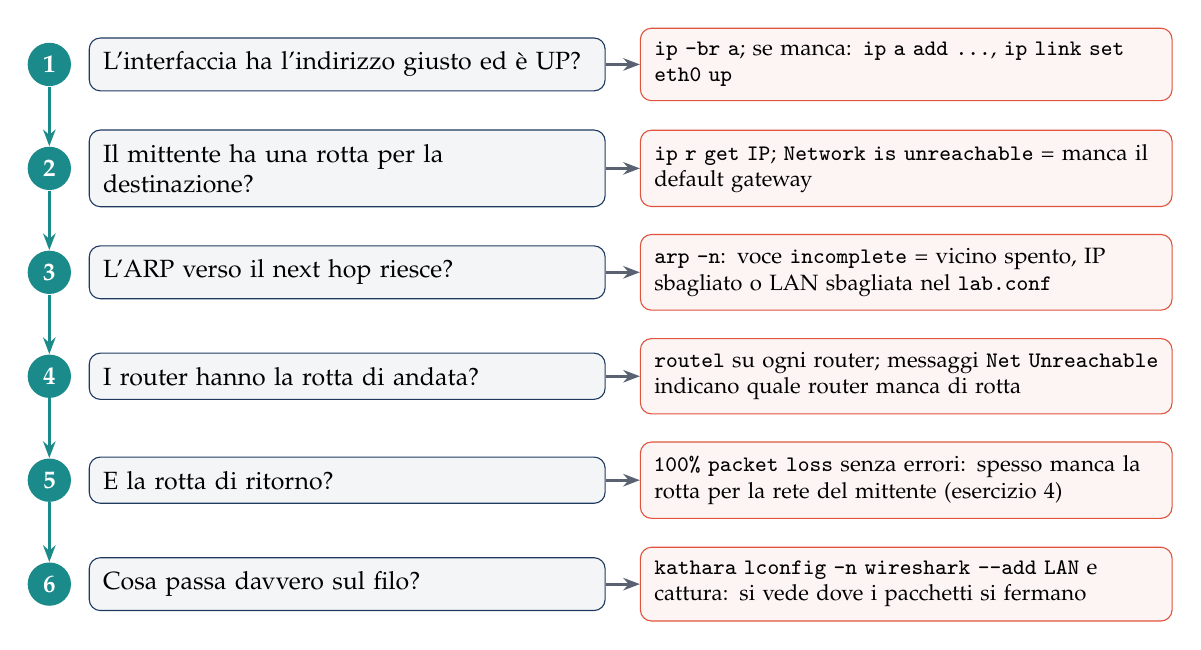
\begin{tikzpicture}[
  st/.style={draw=navy,fill=navy!5,rounded corners=4pt,font=\headfont\small,align=left,text width=6.2cm,inner sep=5pt},
  fx/.style={draw=rosso,fill=rosso!6,rounded corners=4pt,font=\headfont\footnotesize,align=left,text width=6.4cm,inner sep=5pt},
  ar/.style={-{Stealth[length=6pt]},line width=1pt,color=grigio},
  n/.style={circle,fill=teal,text=white,font=\headfont\bfseries\small,inner sep=2pt,minimum size=.55cm}]
  \foreach \i/\q/\f in {
    1/{L'interfaccia ha l'indirizzo giusto ed è UP?}/{\texttt{ip -br a}; se manca: \texttt{ip a add \dots}, \texttt{ip link set eth0 up}},
    2/{Il mittente ha una rotta per la destinazione?}/{\texttt{ip r get IP}; \texttt{Network is unreachable} = manca il default gateway},
    3/{L'ARP verso il next hop riesce?}/{\texttt{arp -n}: voce \texttt{incomplete} = vicino spento, IP sbagliato o LAN sbagliata nel \texttt{lab.conf}},
    4/{I router hanno la rotta di andata?}/{\texttt{routel} su ogni router; messaggi \texttt{Net Unreachable} indicano quale router manca di rotta},
    5/{E la rotta di ritorno?}/{\texttt{100\% packet loss} senza errori: spesso manca la rotta per la rete del mittente (esercizio 4)},
    6/{Cosa passa davvero sul filo?}/{\texttt{kathara lconfig -n wireshark --add LAN} e cattura: si vede dove i pacchetti si fermano}}{
    \node[n] (n\i) at (0,-\i*1.32) {\i};
    \node[st,anchor=west] (q\i) at (.5,-\i*1.32) {\q};
    \node[fx,anchor=west] (f\i) at (7.5,-\i*1.32) {\f};
    \draw[ar] (q\i) -- (f\i);
  }
  \foreach \i [evaluate=\i as \j using int(\i+1)] in {1,...,5}{\draw[ar,teal] (n\i) -- (n\j);}
\end{tikzpicture}
\end{center}

\vspace{4pt}
{\headfont\bfseries\color{navy}Fonti e approfondimenti}
\begin{itemize}
  \item Lab originale: \emph{kathara lab -- basic IPv4 configuration, ping, traceroute and arp}, v3.0, Computer Networks Research Group, Università Roma Tre (\texttt{www.kathara.org}).
  \item Pagine di manuale di Kathará: \texttt{kathara(1)}, \texttt{kathara-lstart(1)}, \texttt{kathara-lconfig(1)}, \texttt{kathara-lab.conf(5)}, \dots{} su \texttt{www.kathara.org/man-pages}.
  \item Repository e documentazione: \texttt{github.com/KatharaFramework/Kathara}.
  \item ARP: RFC 826. ICMP: RFC 792.
\end{itemize}

\end{document}
